% Relatorio do Monte Carlo do rebaixamento rapido do Ceron (Secao 6.1) com o transiente, rodado no PC em 14/11/2026, e
% da amostragem por importancia testada nele. Para refazer (as rodadas pendentes entram sozinhas):
%   python3 -I figuras_rebaixamento.py   (figuras em figs/fig_rb_*.pdf e numeros_rebaixamento.tex; imprime cada numero
%                                         com o arquivo de onde sai)
%   pdflatex relatorio_rebaixamento.tex  (duas vezes)
% Nenhum numero dos dados esta escrito aqui: todos vem das macros do numeros_rebaixamento.tex.
\documentclass[11pt,a4paper]{article}
\usepackage[T1]{fontenc}\usepackage[utf8]{inputenc}\usepackage[brazilian]{babel}\usepackage{lmodern}
\usepackage[margin=2.2cm]{geometry}\usepackage{booktabs}\usepackage{graphicx}\usepackage{caption}
\usepackage{float}\usepackage[hidelinks]{hyperref}\usepackage{amsmath}\usepackage{amssymb}\usepackage{microtype}
\usepackage{array}
\captionsetup{font=small}
\renewcommand{\topfraction}{0.9}\renewcommand{\bottomfraction}{0.8}\renewcommand{\textfraction}{0.07}
\renewcommand{\floatpagefraction}{0.75}
\graphicspath{{figs/}}
% gerado por figuras_rebaixamento.py em 15/11/2026 00:37: nao edite (rode o script de novo)
\newif\ifaipronto \aiprontotrue
\newif\ifmodosdesloc \modosdesloctrue
\newif\ifmodospronto \modosprontotrue
\newif\ifmodosiniciado \modosiniciadotrue
\newif\ifkfixopronto \kfixoprontotrue
\newif\ifkfixoiniciado \kfixoiniciadotrue
\newcommand{\DomX}{70} % rebaixamento_mc.cpp (kTalude)
\newcommand{\DomY}{35} % rebaixamento_mc.cpp (kTalude)
\newcommand{\AlturaH}{5} % rebaixamento_mc.cpp (kTalude)
\newcommand{\Inclinacao}{45} % rebaixamento_mc.cpp (kTalude)
\newcommand{\CristaX}{35} % rebaixamento_mc.cpp (kTalude)
\newcommand{\PeX}{40} % rebaixamento_mc.cpp (kTalude)
\newcommand{\CristaY}{35} % rebaixamento_mc.cpp (kTalude)
\newcommand{\PeY}{30} % rebaixamento_mc.cpp (kTalude)
\newcommand{\Coesao}{10} % rebaixamento_mc.cpp (Solo)
\newcommand{\Atrito}{30} % rebaixamento_mc.cpp (Solo)
\newcommand{\PesoSolo}{20} % rebaixamento_mc.cpp (Solo)
\newcommand{\ModuloE}{20} % rebaixamento_mc.cpp (Solo, MPa)
\newcommand{\Poisson}{0{,}3} % rebaixamento_mc.cpp (Solo)
\newcommand{\Porosidade}{0{,}45} % rebaixamento_mc.cpp (Solo)
\newcommand{\Kv}{10^{-6}} % rebaixamento_mc.cpp (Solo)
\newcommand{\ModuloAgua}{2{,}2} % rebaixamento_mc.cpp (Solo, GPa)
\newcommand{\GammaMain}{1{,}3339} % rebaixamento_mc.cpp (cabecalho: TransientDrawDown do main.cpp)
\newcommand{\NivelMain}{3} % rebaixamento_mc.cpp (cabecalho)
\newcommand{\CovC}{0{,}3} % direto/ceron_tr_fase1/f50_I0_iii/mc_parametros.txt
\newcommand{\CovPhi}{0{,}1} % direto/ceron_tr_fase1/f50_I0_iii/mc_parametros.txt
\newcommand{\CovK}{0{,}6} % direto/ceron_tr_fase1/f50_I0_iii/mc_parametros.txt
\newcommand{\Lx}{20} % direto/ceron_tr_fase1/f50_I0_iii/mc_parametros.txt
\newcommand{\Ly}{2} % direto/ceron_tr_fase1/f50_I0_iii/mc_parametros.txt
\newcommand{\KLM}{2000} % direto/ceron_tr_fase1/f50_I0_iii/mc_parametros.txt
\newcommand{\NVarKL}{6000} % direto/ceron_tr_fase1/f50_I0_iii/mc_parametros.txt (3 campos x KL_M)
\newcommand{\KLvar}{95{,}97} % direto/ceron_tr_fase1/f50_I0_iii/mc_parametros.txt
\newcommand{\Semente}{20250416} % direto/ceron_tr_fase1/f50_I0_iii/mc_parametros.txt
\newcommand{\Trebaix}{0{,}1} % direto/ceron_tr_fase1/f50_I0_iii/mc_parametros.txt
\newcommand{\NivelFinal}{30} % direto/ceron_tr_fase1/f50_I0_iii/mc_parametros.txt
\newcommand{\HwH}{1} % direto/ceron_tr_fase1/f50_I0_iii/mc_parametros.txt
\newcommand{\Nref}{3} % direto/ceron_tr_fase1/f50_I0_iii/mc_parametros.txt
\newcommand{\MalhaT}{tri3} % direto/ceron_tr_fase1/f50_I0_iii/mc_parametros.txt
\newcommand{\MalhaF}{tri1} % direto/ceron_tr_fase1/f50_I0_iii/mc_parametros.txt
\newcommand{\LimiarBanda}{0{,}1} % rebaixamento_mc.cpp (FatorAdaptativo)
\newcommand{\DtTrans}{0{,}1} % DrawdownTransient.h (DrawdownData::dt)
\newcommand{\PassosTrans}{1} % TREBAIX / dt
\newcommand{\TriTrans}{11712} % direto/det/mc_real-1/triangles.csv
\newcommand{\LadoTrans}{0{,}625} % direto/det/mc_real-1/triangles.csv (menor aresta)
\newcommand{\PassoMalha}{5} % direto/det/mc_real-1/triangles.csv (lado x 2^3)
\newcommand{\LadoFator}{2{,}5} % passo / 2^1
\newcommand{\LadoBanda}{0{,}31} % passo / 2^1 / 2^NREF
\newcommand{\GammaDet}{1{,}3253} % direto/det/mc_0_-1.csv
\newcommand{\NiveisDet}{1{,}9137; 1{,}5800; 1{,}3957; 1{,}3253} % direto/det/mc_0_-1.csv
\newcommand{\EqFatorDet}{5786} % direto/det/mc_0_-1.csv
\newcommand{\DifDetCeron}{\ensuremath{-}0{,}80} % direto/det/mc_0_-1.csv e Ceron (Fig. 24)
\newcommand{\GammaCeron}{1{,}336} % Ceron, Fig. 24 (digitado)
\newcommand{\PfCeron}{11{,}50} % Ceron, Tabela 4 (digitado)
\newcommand{\PfCeronS}{21{,}93} % Ceron, Tabela 4 (digitado)
\newcommand{\CovCeron}{23{,}5} % Ceron, Tabela 4 (digitado)
\newcommand{\NCeron}{10\,000} % Ceron, Secao 6.1 (S = 10 000 simulacoes; digitado)
\newcommand{\CovPfCeron}{2{,}77} % Ceron, Secao 6.1 e Tabela 4 (digitado)
\newcommand{\PfCeronLo}{10{,}9} % Ceron, P_f e S (Wilson)
\newcommand{\PfCeronHi}{12{,}1} % Ceron, P_f e S (Wilson)
\newcommand{\GammaMediaCeron}{1{,}353} % Ceron, Tabela 4 (digitado)
\newcommand{\GammaDPCeron}{0{,}318} % Ceron, Tabela 4 (digitado)
\newcommand{\MediaSobreDetCeron}{1{,}3} % Ceron, Tabela 4 e Fig. 24
\newcommand{\PosicaoCeron}{1{,}3\% acima} % Ceron, Tabela 4 e Fig. 24
\newcommand{\PfCeronKfixo}{11{,}21} % Ceron, Tabela 3, CoV(k_v) = 0 (digitado)
\newcommand{\GammaMediaCeronKfixo}{1{,}329} % Ceron, Tabela 3, CoV(k_v) = 0 (digitado)
\newcommand{\CeronDifK}{0{,}29} % Ceron, Tabelas 3 e 4 (pontos)
\newcommand{\NDireto}{2000} % direto/ceron_tr_fase1/f50_I0_iii/mc_*.csv
\newcommand{\NfDireto}{314} % direto/ceron_tr_fase1/f50_I0_iii/mc_*.csv
\newcommand{\PfDireto}{15{,}70} % direto/ceron_tr_fase1/f50_I0_iii/mc_*.csv
\newcommand{\PfDiretoLo}{14{,}2} % direto/ceron_tr_fase1/f50_I0_iii/mc_*.csv (Wilson)
\newcommand{\PfDiretoHi}{17{,}4} % direto/ceron_tr_fase1/f50_I0_iii/mc_*.csv (Wilson)
\newcommand{\CovPfDireto}{5{,}2} % direto/ceron_tr_fase1/f50_I0_iii/mc_*.csv (Eq. 68 do Ceron)
\newcommand{\GammaMedia}{1{,}2941} % direto/ceron_tr_fase1/f50_I0_iii/mc_*.csv
\newcommand{\GammaMediana}{1{,}2586} % direto/ceron_tr_fase1/f50_I0_iii/mc_*.csv
\newcommand{\GammaDP}{0{,}3092} % direto/ceron_tr_fase1/f50_I0_iii/mc_*.csv
\newcommand{\GammaCoV}{23{,}9} % direto/ceron_tr_fase1/f50_I0_iii/mc_*.csv
\newcommand{\GammaMin}{0{,}5835} % direto/ceron_tr_fase1/f50_I0_iii/mc_*.csv
\newcommand{\GammaMax}{3{,}0044} % direto/ceron_tr_fase1/f50_I0_iii/mc_*.csv
\newcommand{\MediaSobreDet}{\ensuremath{-}2{,}4} % direto/ceron_tr_fase1/f50_I0_iii/mc_*.csv
\newcommand{\PosicaoDireto}{2{,}4\% abaixo} % direto/ceron_tr_fase1/f50_I0_iii/mc_*.csv e direto/det/mc_0_-1.csv
\newcommand{\MediaContraCeron}{4{,}4\% abaixo} % direto/ceron_tr_fase1/f50_I0_iii/mc_*.csv e Ceron (Tabela 4)
\newcommand{\LnMu}{0{,}2305} % direto/ceron_tr_fase1/f50_I0_iii/mc_*.csv
\newcommand{\LnSigma}{0{,}2330} % direto/ceron_tr_fase1/f50_I0_iii/mc_*.csv
\newcommand{\PfLogn}{16{,}13} % direto/ceron_tr_fase1/f50_I0_iii/mc_*.csv (ajuste log-normal)
\newcommand{\PfLognCeron}{12{,}2} % direto/ceron_tr_fase1/f50_I0_iii/mc_*.csv (CoV) e Ceron (media, Tabela 4): log-normal
\newcommand{\LillieB}{2000} % bootstrap parametrico (script)
\newcommand{\KSlogD}{0{,}0118} % direto/ceron_tr_fase1/f50_I0_iii/mc_*.csv (Kolmogorov-Smirnov, log-normal)
\newcommand{\KSlogP}{\approx 0{,}76} % direto/ceron_tr_fase1/f50_I0_iii/mc_*.csv (Lilliefors, 2000 amostras)
\newcommand{\KSCritico}{0{,}0202} % Lilliefors: D de 5\% (2000 amostras de n = 2000)
\newcommand{\KSnormD}{0{,}0556} % direto/ceron_tr_fase1/f50_I0_iii/mc_*.csv (Kolmogorov-Smirnov, normal)
\newcommand{\KSnormP}{< 0{,}001} % direto/ceron_tr_fase1/f50_I0_iii/mc_*.csv (Lilliefors, 2000 amostras)
\newcommand{\NPrimeirasQuatrocentas}{400} % janela escolhida no script
\newcommand{\PfPrimeirasQuatrocentas}{18{,}5} % direto/ceron_tr_fase1/f50_I0_iii/mc_*.csv (realizacoes 0..399)
\newcommand{\NPrimeirasMil}{1000} % janela escolhida no script
\newcommand{\PfPrimeirasMil}{16{,}6} % direto/ceron_tr_fase1/f50_I0_iii/mc_*.csv (realizacoes 0..999)
\newcommand{\RhoC}{0{,}85} % direto/ceron_tr_fase1/f50_I0_iii/mc_*.csv (Spearman de Gamma com banda_c)
\newcommand{\FalhaC}{6{,}96} % direto/ceron_tr_fase1/f50_I0_iii/mc_*.csv (media de banda_c nas falhas)
\newcommand{\OutrasC}{9{,}89} % direto/ceron_tr_fase1/f50_I0_iii/mc_*.csv (media de banda_c nas outras)
\newcommand{\DetC}{10{,}00} % direto/det/mc_0_-1.csv (banda_c)
\newcommand{\RhoPhi}{0{,}34} % direto/ceron_tr_fase1/f50_I0_iii/mc_*.csv (Spearman de Gamma com banda_phi_deg)
\newcommand{\FalhaPhi}{28{,}74} % direto/ceron_tr_fase1/f50_I0_iii/mc_*.csv (media de banda_phi_deg nas falhas)
\newcommand{\OutrasPhi}{30{,}00} % direto/ceron_tr_fase1/f50_I0_iii/mc_*.csv (media de banda_phi_deg nas outras)
\newcommand{\DetPhi}{30{,}00} % direto/det/mc_0_-1.csv (banda_phi_deg)
\newcommand{\RhoK}{0{,}22} % direto/ceron_tr_fase1/f50_I0_iii/mc_*.csv (Spearman de Gamma com banda_k_mult)
\newcommand{\FalhaK}{0{,}826} % direto/ceron_tr_fase1/f50_I0_iii/mc_*.csv (media de banda_k_mult nas falhas)
\newcommand{\OutrasK}{0{,}995} % direto/ceron_tr_fase1/f50_I0_iii/mc_*.csv (media de banda_k_mult nas outras)
\newcommand{\DetK}{1{,}000} % direto/det/mc_0_-1.csv (banda_k_mult)
\newcommand{\RhoPw}{\ensuremath{-}0{,}42} % direto/ceron_tr_fase1/f50_I0_iii/mc_*.csv (Spearman de Gamma com banda_pw)
\newcommand{\FalhaPw}{13{,}72} % direto/ceron_tr_fase1/f50_I0_iii/mc_*.csv (media de banda_pw nas falhas)
\newcommand{\OutrasPw}{12{,}09} % direto/ceron_tr_fase1/f50_I0_iii/mc_*.csv (media de banda_pw nas outras)
\newcommand{\DetPw}{12{,}34} % direto/det/mc_0_-1.csv (banda_pw)
\newcommand{\RhoProf}{\ensuremath{-}0{,}33} % direto/ceron_tr_fase1/f50_I0_iii/mc_*.csv (Spearman de Gamma com banda_prof)
\newcommand{\FalhaProf}{2{,}93} % direto/ceron_tr_fase1/f50_I0_iii/mc_*.csv (media de banda_prof nas falhas)
\newcommand{\OutrasProf}{2{,}77} % direto/ceron_tr_fase1/f50_I0_iii/mc_*.csv (media de banda_prof nas outras)
\newcommand{\DetProf}{2{,}66} % direto/det/mc_0_-1.csv (banda_prof)
\newcommand{\ParcC}{0{,}91} % direto/ceron_tr_fase1/f50_I0_iii/mc_*.csv (Spearman parcial de 2a ordem, Eqs. 70-71 do Ceron)
\newcommand{\ParcPhi}{0{,}65} % direto/ceron_tr_fase1/f50_I0_iii/mc_*.csv (Spearman parcial de 2a ordem, Eqs. 70-71 do Ceron)
\newcommand{\ParcK}{0{,}45} % direto/ceron_tr_fase1/f50_I0_iii/mc_*.csv (Spearman parcial de 2a ordem, Eqs. 70-71 do Ceron)
\newcommand{\RhoKPw}{\ensuremath{-}0{,}42} % direto/ceron_tr_fase1/f50_I0_iii/mc_*.csv (Spearman de banda_k_mult com banda_pw)
\newcommand{\RhoPwProf}{0{,}79} % direto/ceron_tr_fase1/f50_I0_iii/mc_*.csv (Spearman de banda_pw com banda_prof)
\newcommand{\MediaNivelZero}{1{,}7984} % direto/ceron_tr_fase1/f50_I0_iii/mc_*.csv (niveis)
\newcommand{\PfNivelZero}{0{,}65} % direto/ceron_tr_fase1/f50_I0_iii/mc_*.csv (niveis)
\newcommand{\DetNivelZero}{1{,}9137} % direto/det/mc_0_-1.csv (niveis)
\newcommand{\MediaNivelUm}{1{,}4899} % direto/ceron_tr_fase1/f50_I0_iii/mc_*.csv (niveis)
\newcommand{\PfNivelUm}{6{,}05} % direto/ceron_tr_fase1/f50_I0_iii/mc_*.csv (niveis)
\newcommand{\DetNivelUm}{1{,}5800} % direto/det/mc_0_-1.csv (niveis)
\newcommand{\MediaNivelDois}{1{,}3503} % direto/ceron_tr_fase1/f50_I0_iii/mc_*.csv (niveis)
\newcommand{\PfNivelDois}{11{,}80} % direto/ceron_tr_fase1/f50_I0_iii/mc_*.csv (niveis)
\newcommand{\DetNivelDois}{1{,}3957} % direto/det/mc_0_-1.csv (niveis)
\newcommand{\MediaNivelTres}{1{,}2941} % direto/ceron_tr_fase1/f50_I0_iii/mc_*.csv (niveis)
\newcommand{\PfNivelTres}{15{,}70} % direto/ceron_tr_fase1/f50_I0_iii/mc_*.csv (niveis)
\newcommand{\DetNivelTres}{1{,}3253} % direto/det/mc_0_-1.csv (niveis)
\newcommand{\UltimoNivel}{\ensuremath{-}4{,}1} % direto/ceron_tr_fase1/f50_I0_iii/mc_*.csv (Gamma_3 / Gamma_2 - 1, media)
\newcommand{\UltimoNivelDet}{\ensuremath{-}5{,}0} % direto/det/mc_0_-1.csv
\newcommand{\RazaoNiveis}{0{,}40} % direto/ceron_tr_fase1/f50_I0_iii/mc_*.csv (razao das duas ultimas variacoes da media)
\newcommand{\ExtrapQuatro}{\ensuremath{-}1{,}7} % extrapolacao geometrica das medias por nivel
\newcommand{\ExtrapLimite}{\ensuremath{-}2{,}9} % extrapolacao geometrica das medias por nivel
\newcommand{\PfExtrapQuatro}{17{,}8} % direto/ceron_tr_fase1/f50_I0_iii/mc_*.csv (Gamma x (1 + extrapolacao) < 1)
\newcommand{\PfExtrapLimite}{19{,}6} % direto/ceron_tr_fase1/f50_I0_iii/mc_*.csv (Gamma x (1 + extrapolacao) < 1)
\newcommand{\PfMenosUm}{16{,}7} % direto/ceron_tr_fase1/f50_I0_iii/mc_*.csv (Gamma x 0.99 < 1)
\newcommand{\PfMenosDois}{18{,}1} % direto/ceron_tr_fase1/f50_I0_iii/mc_*.csv (Gamma x 0.98 < 1)
\newcommand{\EqFatorMin}{4978} % direto/ceron_tr_fase1/f50_I0_iii/mc_*.csv
\newcommand{\EqFatorMax}{8078} % direto/ceron_tr_fase1/f50_I0_iii/mc_*.csv
\newcommand{\EqTrans}{59548} % direto/ceron_tr_fase1/f50_I0_iii/mc_*.csv
\newcommand{\CustoReal}{37{,}2} % direto/ceron_tr_fase1/f50_I0_iii/mc_*.log (tempo por realizacao)
\newcommand{\CustoMediana}{35{,}4} % direto/ceron_tr_fase1/f50_I0_iii/mc_*.log
\newcommand{\CustoTrans}{15{,}0} % direto/ceron_tr_fase1/f50_I0_iii/mc_*.log (transiente)
\newcommand{\CustoFator}{20{,}7} % direto/ceron_tr_fase1/f50_I0_iii/mc_*.csv (s_fator)
\newcommand{\CustoResto}{1{,}5} % direto/ceron_tr_fase1/f50_I0_iii/mc_*.log e mc_*.csv (total - transiente - s_fator)
\newcommand{\CustoPrimeiras}{34{,}7} % direto/ceron_tr_fase1/f50_I0_iii/mc_*.log (realizacoes 0..399)
\newcommand{\CustoUltimas}{38{,}2} % direto/ceron_tr_fase1/f50_I0_iii/mc_*.log (realizacoes 1600..1999)
\newcommand{\ProcPC}{8} % direto/rodar.sh
\newcommand{\RelogioDireto}{2~h 37~min} % direto/logs/pp*.txt
\newcommand{\InicioDireto}{16h57} % direto/logs/pp*.txt
\newcommand{\FimDireto}{19h34} % direto/logs/pp*.txt
\newcommand{\RelogioPorReal}{4{,}7} % direto/logs/pp*.txt / N
\newcommand{\CelulasMapa}{44} % direto/ceron_tr_fase1/f50_I0_iii/mc_mapa_*.csv
\newcommand{\CelulasMetade}{11} % direto/ceron_tr_fase1/f50_I0_iii/mc_mapa_*.csv (celulas com a banda em >= 50\% das realizacoes)
\newcommand{\CelulasMetadeFalha}{11} % direto/ceron_tr_fase1/f50_I0_iii/mc_mapa_*.csv (o mesmo nas falhas)
\newcommand{\DifDetMain}{\ensuremath{-}0{,}64} % direto/det/mc_0_-1.csv e rebaixamento_mc.cpp
\newcommand{\AguaAntiga}{percolacao\_permanente} % ceron_mc/ceron_mc_fase1/f50_I0_iii/parametros.txt
\newcommand{\MalhaAntiga}{ceron\_h5\_a45\_g15.msh} % ceron_mc/ceron_mc_fase1/f50_I0_iii/parametros.txt
\newcommand{\NrefAntiga}{3} % ceron_mc/ceron_mc_fase1/f50_I0_iii/parametros.txt
\newcommand{\PmaxAntiga}{2} % ceron_mc/ceron_mc_fase1/f50_I0_iii/parametros.txt
\newcommand{\NAntiga}{5770} % ceron_mc/ceron_mc_fase1/f50_I0_iii/mc_resumo.csv
\newcommand{\NfAntiga}{540} % ceron_mc/ceron_mc_fase1/f50_I0_iii/mc_resumo.csv
\newcommand{\PfAntiga}{9{,}36} % ceron_mc/ceron_mc_fase1/f50_I0_iii/mc_resumo.csv
\newcommand{\PfAntigaLo}{8{,}6} % ceron_mc/ceron_mc_fase1/f50_I0_iii/mc_resumo.csv (Wilson)
\newcommand{\PfAntigaHi}{10{,}1} % ceron_mc/ceron_mc_fase1/f50_I0_iii/mc_resumo.csv (Wilson)
\newcommand{\GammaMediaAntiga}{1{,}3958} % ceron_mc/ceron_mc_fase1/f50_I0_iii/mc_resumo.csv
\newcommand{\GammaCoVAntiga}{24{,}2} % ceron_mc/ceron_mc_fase1/f50_I0_iii/mc_resumo.csv
\newcommand{\GammaMedianaAntiga}{1{,}3539} % ceron_mc/ceron_mc_fase1/f50_I0_iii/mc_resumo.csv
\newcommand{\GammaDetAntiga}{1{,}4032} % ceron_mc/ceron_mc_fase1/f50_I0_iii_det/r00000/gim_unsat.csv
\newcommand{\MediaSobreDetAntiga}{\ensuremath{-}0{,}5} % ceron_mc/ceron_mc_fase1/f50_I0_iii/mc_resumo.csv
\newcommand{\DomXAntiga}{25} % Projects/LearningMohrCoulomb2/cluster/malhas/ceron_h5_a45_g15.msh (caixa dos nos)
\newcommand{\DomYAntiga}{10} % Projects/LearningMohrCoulomb2/cluster/malhas/ceron_h5_a45_g15.msh (caixa dos nos)
\newcommand{\KLvarAntiga}{99{,}20} % ceron_mc/ceron_mc_fase1/f50_I0_iii/mc_resumo.csv (KL_variancia)
\newcommand{\AreaAntiga}{187{,}5} % ceron_mc/ceron_mc_fase1/f50_I0_iii/mc_resumo.csv (area_solo_m2)
\newcommand{\NComuns}{2000} % ceron_mc/ceron_mc_fase1/f50_I0_iii/mc_resumo.csv e direto
\newcommand{\CorrCmed}{0{,}92} % ceron_mc/ceron_mc_fase1/f50_I0_iii/mc_resumo.csv e direto (Pearson de c_med, mesmo n)
\newcommand{\CorrPhimed}{0{,}93} % ceron_mc/ceron_mc_fase1/f50_I0_iii/mc_resumo.csv e direto (Pearson de phi_med, mesmo n)
\newcommand{\CorrKmed}{0{,}92} % ceron_mc/ceron_mc_fase1/f50_I0_iii/mc_resumo.csv e direto (Pearson de k_mult_med, mesmo n)
\newcommand{\CorrBandaC}{0{,}03} % ceron_mc/ceron_mc_fase1/f50_I0_iii/mc_resumo.csv e direto (Pearson de banda_c, mesmo n)
\newcommand{\CorrGamma}{0{,}08} % ceron_mc/ceron_mc_fase1/f50_I0_iii/mc_resumo.csv e direto (Pearson de FS_min, mesmo n)
\newcommand{\PfAntigaComuns}{9{,}55} % ceron_mc/ceron_mc_fase1/f50_I0_iii/mc_resumo.csv (as realizacoes 0..1999)
\newcommand{\PfAntigaNivelZero}{1{,}18} % ceron_mc/ceron_mc_fase1/f50_I0_iii/mc_resumo.csv (gamma_nivel0)
\newcommand{\PfAntigaNivelUm}{4{,}09} % ceron_mc/ceron_mc_fase1/f50_I0_iii/mc_resumo.csv (gamma_nivel1)
\newcommand{\PfAntigaNivelDois}{7{,}37} % ceron_mc/ceron_mc_fase1/f50_I0_iii/mc_resumo.csv (gamma_nivel2)
\newcommand{\PfAntigaNivelTres}{9{,}36} % ceron_mc/ceron_mc_fase1/f50_I0_iii/mc_resumo.csv (gamma_nivel3)
\newcommand{\AntNPar}{5709} % ceron_mc/ceron_mc_fase2/f50_I0_iii_covk0/mc_resumo.csv e ceron_mc/ceron_mc_fase1/f50_I0_iii/mc_resumo.csv
\newcommand{\AntPfFixo}{9{,}13} % ceron_mc/ceron_mc_fase2/f50_I0_iii_covk0/mc_resumo.csv e ceron_mc/ceron_mc_fase1/f50_I0_iii/mc_resumo.csv
\newcommand{\AntPfAleat}{9{,}32} % ceron_mc/ceron_mc_fase2/f50_I0_iii_covk0/mc_resumo.csv e ceron_mc/ceron_mc_fase1/f50_I0_iii/mc_resumo.csv
\newcommand{\AntNzu}{119} % ceron_mc/ceron_mc_fase2/f50_I0_iii_covk0/mc_resumo.csv e ceron_mc/ceron_mc_fase1/f50_I0_iii/mc_resumo.csv (so com k aleatorio)
\newcommand{\AntNuz}{108} % ceron_mc/ceron_mc_fase2/f50_I0_iii_covk0/mc_resumo.csv e ceron_mc/ceron_mc_fase1/f50_I0_iii/mc_resumo.csv (so com k fixo)
\newcommand{\AntMcNemar}{= 0{,}51} % ceron_mc/ceron_mc_fase2/f50_I0_iii_covk0/mc_resumo.csv e ceron_mc/ceron_mc_fase1/f50_I0_iii/mc_resumo.csv (McNemar)
\newcommand{\AntDifGamma}{0{,}0186} % ceron_mc/ceron_mc_fase2/f50_I0_iii_covk0/mc_resumo.csv e ceron_mc/ceron_mc_fase1/f50_I0_iii/mc_resumo.csv (Gamma(aleatorio) - Gamma(fixo))
\newcommand{\AntDifGammaSe}{0{,}0015} % ceron_mc/ceron_mc_fase2/f50_I0_iii_covk0/mc_resumo.csv e ceron_mc/ceron_mc_fase1/f50_I0_iii/mc_resumo.csv
\newcommand{\BetaLinear}{1{,}01} % formula (relatorio_chuva.tex, Secao 7), P_f do direto
\newcommand{\MdoisLinear}{2{,}34} % formula, P_f do direto
\newcommand{\GanhoLinear}{4{,}0} % formula, P_f do direto
\newcommand{\PfChuva}{1} % cluster/README.md (pilotos do relatorio_chuva.tex)
\newcommand{\GanhoLinearUm}{37{,}5} % formula, P_f da chuva
\newcommand{\SC}{\ensuremath{-}1{,}30} % ai/desloc.txt
\newcommand{\SPhi}{\ensuremath{-}0{,}49} % ai/desloc.txt
\newcommand{\SK}{\ensuremath{-}0{,}36} % ai/desloc.txt
\newcommand{\MuDoisBanda}{2{,}06} % ai/desloc.txt
\newcommand{\VarPesoBanda}{6{,}89} % exp(|mu|^2) - 1
\newcommand{\RuidoBanda}{0{,}010} % 3 / n_f
\newcommand{\NAlvoBanda}{1000} % ai/casos.txt
\newcommand{\SementeBanda}{1} % ai/casos.txt
\newcommand{\GammaDetBanda}{1{,}3253} % ai/ceron_tr_fase1_ai/f50_I0_iii/mc_0_49.csv
\newcommand{\NBanda}{1000} % ai/ceron_tr_fase1_ai/f50_I0_iii/mc_*.csv
\newcommand{\SemFatorBanda}{0} % ai/ceron_tr_fase1_ai/f50_I0_iii/mc_*.csv
\newcommand{\PfBanda}{15{,}87} % ai/ceron_tr_fase1_ai/f50_I0_iii/mc_*.csv (soma(peso * falha) / N)
\newcommand{\CovPfBanda}{4{,}4} % ai/ceron_tr_fase1_ai/f50_I0_iii/mc_*.csv
\newcommand{\PfBandaLo}{14{,}5} % ai/ceron_tr_fase1_ai/f50_I0_iii/mc_*.csv (P_f (1 -+ 1,96 CoV))
\newcommand{\PfBandaHi}{17{,}2} % ai/ceron_tr_fase1_ai/f50_I0_iii/mc_*.csv
\newcommand{\NfBanda}{626} % ai/ceron_tr_fase1_ai/f50_I0_iii/mc_*.csv (falhas sorteadas)
\newcommand{\FracFalhaBanda}{63} % ai/ceron_tr_fase1_ai/f50_I0_iii/mc_*.csv
\newcommand{\PesoMedioBanda}{0{,}945} % ai/ceron_tr_fase1_ai/f50_I0_iii/mc_*.csv
\newcommand{\PesoMedioBandaSe}{0{,}060} % ai/ceron_tr_fase1_ai/f50_I0_iii/mc_*.csv
\newcommand{\EssBanda}{201} % ai/ceron_tr_fase1_ai/f50_I0_iii/mc_*.csv ((soma w)^2 / soma w^2)
\newcommand{\PesoFalhaBanda}{0{,}25} % ai/ceron_tr_fase1_ai/f50_I0_iii/mc_*.csv (peso medio nas falhas)
\newcommand{\PesoMaxBanda}{1{,}45} % ai/ceron_tr_fase1_ai/f50_I0_iii/mc_*.csv (maior peso nas falhas)
\newcommand{\ProjMediaBanda}{\ensuremath{-1{,}30;\ -0{,}46;\ -0{,}35}} % ai/ceron_tr_fase1_ai/f50_I0_iii/mc_*.csv (media de proj_* sorteadas)
\newcommand{\DifBanda}{0{,}16} % ai/ceron_tr_fase1_ai/f50_I0_iii/mc_*.csv e direto/ceron_tr_fase1/f50_I0_iii/mc_*.csv (desvios)
\newcommand{\DifBandaPontos}{0{,}17} % ai/ceron_tr_fase1_ai/f50_I0_iii/mc_*.csv e direto/ceron_tr_fase1/f50_I0_iii/mc_*.csv
\newcommand{\GanhoBanda}{2{,}7} % ai/ceron_tr_fase1_ai/f50_I0_iii/mc_*.csv ((CoV do direto com N e P_f da AI / CoV da AI)^2)
\newcommand{\CovDiretoMesmoNBanda}{7{,}3} % Eq. 68 com N e P_f da AI
\newcommand{\FracGanhoBanda}{69} % ganho medido / ganho linear
\newcommand{\NDiretoParaCovBanda}{2711} % Eq. 68 com o CoV da AI
\newcommand{\ViesBanda}{sem sinal de viés, abaixo de dois desvios} % ai/ceron_tr_fase1_ai/f50_I0_iii/mc_*.csv
\newcommand{\CustoBanda}{31{,}1} % ai/ceron_tr_fase1_ai/f50_I0_iii/mc_*.log
\newcommand{\InicioBanda}{19h35} % ai/logs/pp*.txt
\newcommand{\FimBanda}{20h53} % ai/logs/pp*.txt
\newcommand{\RelogioBanda}{1~h 18~min} % ai/logs/pp*.txt
\newcommand{\KModos}{20} % ai_modos/cadeia2.sh
\newcommand{\NAlvoModos}{1000} % ai_modos/cadeia2.sh
\newcommand{\SementeModos}{2} % ai_modos/cadeia2.sh
\newcommand{\RuidoModos}{0{,}19} % 3K / n_f
\newcommand{\FatorRuidoModos}{1{,}21} % exp(3K / n_f)
\newcommand{\DirecaoK}{65} % verificacao/banda_direcao.csv
\newcommand{\MuDoisModos}{1{,}67} % ai_modos/modos_desloc_modos.csv
\newcommand{\MuDoisModosUtil}{0{,}92} % ai_modos/modos_desloc_modos.csv e verificacao/banda_direcao.csv
\newcommand{\MuDoisModosResto}{0{,}75} % ai_modos/modos_desloc_modos.csv e verificacao/banda_direcao.csv
\newcommand{\FatorRestoModos}{2{,}1} % exp(resto)
\newcommand{\FalhasModos}{314} % ai_modos/falhas.txt
\newcommand{\MuDoisVerif}{2{,}15} % verificacao/modos_desloc_1000000_1019999.txt
\newcommand{\MuDoisVerifUtil}{0{,}94} % verificacao/modos_desloc_1000000_1019999.txt e banda_direcao.csv
\newcommand{\PilotoVerif}{400} % verificacao/modos_desloc_1000000_1019999.txt
\newcommand{\FalhasVerif}{74} % verificacao/modos_desloc_1000000_1019999.txt
\newcommand{\SorteiosBanda}{20\,000} % verificacao/banda_*
\newcommand{\PesoVerifBanda}{1{,}007} % verificacao/banda_*
\newcommand{\PesoVerifSeBanda}{0{,}020} % verificacao/banda_*
\newcommand{\VarVerifBanda}{8{,}21} % verificacao/banda_*
\newcommand{\VarTeorBanda}{7{,}54} % verificacao/banda_* (exp(|mu|^2) - 1)
\newcommand{\SorteiosModos}{20\,000} % verificacao/modos_*
\newcommand{\PesoVerifModos}{1{,}008} % verificacao/modos_*
\newcommand{\PesoVerifSeModos}{0{,}020} % verificacao/modos_*
\newcommand{\VarVerifModos}{8{,}07} % verificacao/modos_*
\newcommand{\VarTeorModos}{7{,}59} % verificacao/modos_* (exp(|mu|^2) - 1)
\newcommand{\NModos}{1000} % ai_modos/ceron_tr_fase1_ai_modos/f50_I0_iii/mc_*.csv
\newcommand{\SemFatorModos}{0} % ai_modos/ceron_tr_fase1_ai_modos/f50_I0_iii/mc_*.csv
\newcommand{\PfModos}{17{,}89} % ai_modos/ceron_tr_fase1_ai_modos/f50_I0_iii/mc_*.csv (soma(peso * falha) / N)
\newcommand{\CovPfModos}{6{,}2} % ai_modos/ceron_tr_fase1_ai_modos/f50_I0_iii/mc_*.csv
\newcommand{\NfModos}{509} % ai_modos/ceron_tr_fase1_ai_modos/f50_I0_iii/mc_*.csv
\newcommand{\FracFalhaModos}{51} % ai_modos/ceron_tr_fase1_ai_modos/f50_I0_iii/mc_*.csv
\newcommand{\PesoMedioModos}{0{,}933} % ai_modos/ceron_tr_fase1_ai_modos/f50_I0_iii/mc_*.csv
\newcommand{\PesoMedioModosSe}{0{,}050} % ai_modos/ceron_tr_fase1_ai_modos/f50_I0_iii/mc_*.csv
\newcommand{\EssModos}{262} % ai_modos/ceron_tr_fase1_ai_modos/f50_I0_iii/mc_*.csv
\newcommand{\PesoFalhaModos}{0{,}35} % ai_modos/ceron_tr_fase1_ai_modos/f50_I0_iii/mc_*.csv
\newcommand{\PesoMaxModos}{4{,}28} % ai_modos/ceron_tr_fase1_ai_modos/f50_I0_iii/mc_*.csv
\newcommand{\DifModos}{1{,}58} % ai_modos/ceron_tr_fase1_ai_modos/f50_I0_iii/mc_*.csv e direto/ceron_tr_fase1/f50_I0_iii/mc_*.csv (desvios)
\newcommand{\GanhoModos}{1{,}2} % ai_modos/ceron_tr_fase1_ai_modos/f50_I0_iii/mc_*.csv
\newcommand{\CovDiretoMesmoNModos}{6{,}8} % Eq. 68 com N e P_f da AI
\newcommand{\ViesModos}{sem sinal de viés, abaixo de dois desvios} % ai_modos/ceron_tr_fase1_ai_modos/f50_I0_iii/mc_*.csv
\newcommand{\ComparaGanho}{menor que} % ai_modos/ceron_tr_fase1_ai_modos/f50_I0_iii/mc_*.csv e ai/ceron_tr_fase1_ai/f50_I0_iii/mc_*.csv
\newcommand{\InicioModos}{20h54} % ai_modos/logs/pp*.txt
\newcommand{\FimModos}{22h13} % ai_modos/logs/pp*.txt
\newcommand{\NAlvoKfixo}{2000} % covk0/casos.txt
\newcommand{\CovKfixo}{0} % covk0/casos.txt
\newcommand{\KNPar}{2000} % covk0/ceron_tr_covk0/f50_I0_iii/mc_*.csv e direto
\newcommand{\KSemFator}{0} % covk0/ceron_tr_covk0/f50_I0_iii/mc_*.csv
\newcommand{\KPfFixo}{13{,}80} % covk0/ceron_tr_covk0/f50_I0_iii/mc_*.csv e direto
\newcommand{\KPfFixoLo}{12{,}4} % covk0/ceron_tr_covk0/f50_I0_iii/mc_*.csv e direto (Wilson)
\newcommand{\KPfFixoHi}{15{,}4} % covk0/ceron_tr_covk0/f50_I0_iii/mc_*.csv e direto (Wilson)
\newcommand{\KPfAleat}{15{,}70} % covk0/ceron_tr_covk0/f50_I0_iii/mc_*.csv e direto
\newcommand{\KPfAleatLo}{14{,}2} % covk0/ceron_tr_covk0/f50_I0_iii/mc_*.csv e direto (Wilson)
\newcommand{\KPfAleatHi}{17{,}4} % covk0/ceron_tr_covk0/f50_I0_iii/mc_*.csv e direto (Wilson)
\newcommand{\KNzu}{88} % covk0/ceron_tr_covk0/f50_I0_iii/mc_*.csv e direto (so com k aleatorio)
\newcommand{\KNuz}{50} % covk0/ceron_tr_covk0/f50_I0_iii/mc_*.csv e direto (so com k fixo)
\newcommand{\KMcNemar}{= 0{,}002} % covk0/ceron_tr_covk0/f50_I0_iii/mc_*.csv e direto (McNemar, com a relacao)
\newcommand{\KDifPf}{1{,}90} % covk0/ceron_tr_covk0/f50_I0_iii/mc_*.csv e direto (pontos)
\newcommand{\KDifPfSe}{0{,}59} % covk0/ceron_tr_covk0/f50_I0_iii/mc_*.csv e direto (pontos)
\newcommand{\KDifGamma}{0{,}0037} % covk0/ceron_tr_covk0/f50_I0_iii/mc_*.csv e direto
\newcommand{\KDifGammaSe}{0{,}0026} % covk0/ceron_tr_covk0/f50_I0_iii/mc_*.csv e direto
\newcommand{\KDifGammaMediana}{\ensuremath{-}0{,}0057} % covk0/ceron_tr_covk0/f50_I0_iii/mc_*.csv e direto
\newcommand{\KMaisAleat}{47} % covk0/ceron_tr_covk0/f50_I0_iii/mc_*.csv e direto (\% com Gamma maior com k aleatorio)
\newcommand{\KRhoBanda}{0{,}63} % covk0/ceron_tr_covk0/f50_I0_iii/mc_*.csv e direto (Spearman da diferenca com banda_k_mult)
\newcommand{\KRhoSolo}{0{,}11} % covk0/ceron_tr_covk0/f50_I0_iii/mc_*.csv e direto (Spearman da diferenca com k_mult_med)
\newcommand{\KGammaDet}{1{,}3253} % covk0/ceron_tr_covk0/f50_I0_iii/mc_0_49.csv
\newcommand{\KConclusao}{A diferença é significativa: com o $k_v$ aleatório a $P_f$ sobe, e o $k_v$ explica parte da $P_f$ maior do transiente.} % covk0/ceron_tr_covk0/f50_I0_iii/mc_*.csv e direto (McNemar p < 0,05?)
\newcommand{\InicioKfixo}{22h13} % covk0/cadeia3.log
\newcommand{\FimKfixo}{0h37 de 15/11} % covk0/cadeia3.log
\newcommand{\SolosHora}{20h24} % status.sh no fermi as 20h24 (digitado)
\newcommand{\SolosInicio}{19h21} % status.sh no fermi as 20h24 (digitado)
\newcommand{\SolosNos}{4} % status.sh no fermi as 20h24 (digitado)
\newcommand{\SolosPrevMin}{17} % status.sh no fermi as 20h24 (digitado)
\newcommand{\SolosPrevMax}{20} % status.sh no fermi as 20h24 (digitado)
\newcommand{\SolosFimFaixa}{13h30 e 16h30 de 15/11} % status.sh no fermi as 20h24 (digitado) + previsao
\newcommand{\SolosNDez}{1000} % cluster/casos_solos.txt
\newcommand{\SolosTemposDez}{6, 12, 18, 24, 30, 36, 42, 48} % cluster/casos_solos.txt
\newcommand{\SolosFeitasDez}{63} % status.sh no fermi as 20h24 (digitado)
\newcommand{\SolosFalhasDez}{61} % status.sh no fermi as 20h24 (digitado)
\newcommand{\SolosPfDez}{96{,}83} % status.sh no fermi as 20h24 (digitado)
\newcommand{\SolosLoDez}{89{,}1} % status.sh no fermi as 20h24 (digitado) (Wilson)
\newcommand{\SolosHiDez}{99{,}1} % status.sh no fermi as 20h24 (digitado) (Wilson)
\newcommand{\SolosDetDez}{0{,}832} % status.sh no fermi as 20h24 (digitado)
\newcommand{\SolosTdetDez}{12 a 24~h} % status.sh no fermi as 20h24 (digitado)
\newcommand{\SolosNCinquenta}{1000} % cluster/casos_solos.txt
\newcommand{\SolosTemposCinquenta}{0, 6, 12, 18, 24, 30, 36, 42, 48} % cluster/casos_solos.txt
\newcommand{\SolosFeitasCinquenta}{81} % status.sh no fermi as 20h24 (digitado)
\newcommand{\SolosFalhasCinquenta}{14} % status.sh no fermi as 20h24 (digitado)
\newcommand{\SolosPfCinquenta}{17{,}28} % status.sh no fermi as 20h24 (digitado)
\newcommand{\SolosLoCinquenta}{10{,}6} % status.sh no fermi as 20h24 (digitado) (Wilson)
\newcommand{\SolosHiCinquenta}{26{,}9} % status.sh no fermi as 20h24 (digitado) (Wilson)
\newcommand{\SolosDetCinquenta}{1{,}035} % status.sh no fermi as 20h24 (digitado)
\newcommand{\SolosTdetCinquenta}{24~h} % status.sh no fermi as 20h24 (digitado)
\newcommand{\SolosNCem}{1000} % cluster/casos_solos.txt
\newcommand{\SolosTemposCem}{6, 12, 18, 24, 30, 36, 42, 48} % cluster/casos_solos.txt
\newcommand{\SolosFeitasCem}{75} % status.sh no fermi as 20h24 (digitado)
\newcommand{\SolosFalhasCem}{0} % status.sh no fermi as 20h24 (digitado)
\newcommand{\SolosPfCem}{0{,}00} % status.sh no fermi as 20h24 (digitado)
\newcommand{\SolosLoCem}{0{,}0} % status.sh no fermi as 20h24 (digitado) (Wilson)
\newcommand{\SolosHiCem}{4{,}9} % status.sh no fermi as 20h24 (digitado) (Wilson)
\newcommand{\SolosDetCem}{1{,}881} % status.sh no fermi as 20h24 (digitado)
\newcommand{\SolosTdetCem}{36~h} % status.sh no fermi as 20h24 (digitado)
\newcommand{\SolosIks}{1} % cluster/casos_solos.txt
\newcommand{\SolosDuracao}{24} % cluster/casos_solos.txt
\newcommand{\SolosPasso}{6} % cluster/casos_solos.txt (tempos)
\newcommand{\SolosFim}{48} % cluster/casos_solos.txt (tempos)
\newcommand{\SolosIDez}{360} % cluster/casos_solos.txt
\newcommand{\SolosICinquenta}{36} % cluster/casos_solos.txt
\newcommand{\SolosICem}{3{,}6} % cluster/casos_solos.txt
\newcommand{\SolosTotal}{3000} % cluster/casos_solos.txt
\newcommand{\SolosFeitasTotal}{219} % status.sh no fermi as 20h24 (digitado)
\newcommand{\SolosMinReal}{22} % cluster/README.md
\newcommand{\Nos}{4} % cluster/submeter.sh
\newcommand{\Paralelo}{12} % cluster/submeter.sh
\newcommand{\FermiLento}{2{,}6} % medido antes (digitado)
\newcommand{\CustoFermi}{97} % custo do PC x 2,6
\newcommand{\CeronDireto}{10\,000} % cluster/casos_ceron.txt
\newcommand{\CeronBanda}{5000} % cluster/casos_ceron.txt
\newcommand{\CeronModos}{5000} % cluster/casos_ceron.txt
\newcommand{\CeronTotal}{20\,000} % cluster/casos_ceron.txt
\newcommand{\CeronCpu}{537} % casos_ceron.txt x custo no fermi
\newcommand{\CeronRelogio}{11} % CPU / (4 x 12)
\newcommand{\CeronPiloto}{1000} % cluster/casos_ceron.txt
\newcommand{\CeronPilotoFalhas}{157} % piloto_n x P_f do direto (esperado)
\newcommand{\ChuvaAIPiloto}{200} % cluster/casos_chuva_ai.txt
\newcommand{\ChuvaAIN}{200} % cluster/casos_chuva_ai.txt
\newcommand{\ChuvaAITempos}{6 a 48} % cluster/casos_chuva_ai.txt
\newcommand{\ChuvaAIPasso}{6} % cluster/casos_chuva_ai.txt
\newcommand{\ChuvaAIFim}{48} % cluster/casos_chuva_ai.txt
\newcommand{\ChuvaAIMin}{17} % cluster/casos_chuva_ai.txt
\newcommand{\ChuvaAIRodadas}{10} % casos_chuva_ai.txt: ceil(piloto / 48) + ceil(AI / 48)
\newcommand{\ChuvaAIRelogio}{2{,}8} % rodadas x 17 min
\newcommand{\ChuvaAICovLin}{14} % cluster/README.md
\newcommand{\ChuvaAICovMax}{25} % cluster/README.md
\newcommand{\Iref}{31{,}05} % cluster/campanha.sh
\newcommand{\ChuvaRefTempos}{0 a 24} % cluster/casos.txt (ref)
\newcommand{\ChuvaFaseUmN}{5000} % cluster/casos.txt
\newcommand{\ChuvaFaseUmCasos}{1} % cluster/casos.txt
\newcommand{\ChuvaFaseUmCpu}{866} % cluster/casos.txt + mc/serial_I24.log x 2,6
\newcommand{\ChuvaFaseUmRelogio}{18{,}0} % CPU / 48 processos
\newcommand{\ChuvaFaseDoisN}{40\,000} % cluster/casos.txt
\newcommand{\ChuvaFaseDoisCasos}{20} % cluster/casos.txt
\newcommand{\ChuvaFaseDoisCpu}{2891} % cluster/casos.txt + mc/serial_I24.log x 2,6
\newcommand{\ChuvaFaseDoisRelogio}{60{,}2} % CPU / 48 processos
\newcommand{\ChuvaFaseTresN}{12\,000} % cluster/casos.txt
\newcommand{\ChuvaFaseTresCasos}{6} % cluster/casos.txt
\newcommand{\ChuvaFaseTresCpu}{653} % cluster/casos.txt + mc/serial_I24.log x 2,6
\newcommand{\ChuvaFaseTresRelogio}{13{,}6} % CPU / 48 processos
\newcommand{\ChuvaTotalDias}{3{,}8} % cluster/casos.txt + mc/serial_I24.log
\newcommand{\ChuvaRelogioFaseUmReadme}{21} % cluster/README.md
\newcommand{\SugCasos}{21} % pastas f50_I0_iii_* da campanha antiga, sem os covk*
\newcommand{\SugNporCaso}{2000} % sugestao
\newcommand{\SugBCpu}{1127} % casos x 2000 x custo no fermi (nref = 3)
\newcommand{\SugBRelogio}{23} % CPU / 48 processos
\newcommand{\SugBCpuQuatro}{1800} % o mesmo com o custo de nref = 4 (estimado)
\newcommand{\SugBRelogioQuatro}{37} % CPU / 48 processos
\newcommand{\SugLimiar}{3} % sugestao
\newcommand{\SugPequenos}{5} % campanha antiga: P_f < 3\%
\newcommand{\SugPequenosLista}{$CoV(c') = 0{,}1$ com 0{,}16\%, $h_w/H = 0{,}5$ com 1{,}20\%, $\alpha = 5$ com 1{,}54\%, $\alpha = 4$ com 1{,}85\% e $\alpha = 3$ com 2{,}67\%} % campanha antiga (mc_resumo.csv de cada caso)
\newcommand{\SugDiretos}{16} % campanha antiga: P_f >= 3\%
\newcommand{\SugPfMaxAntiga}{37{,}5} % campanha antiga
\newcommand{\SugPfMinDireto}{3{,}4} % campanha antiga
\newcommand{\SugCovPfMax}{12} % Eq. 68, N = 2000
\newcommand{\SugMalhaN}{50} % sugestao
\newcommand{\SugMalhaBloco}{7} % ceil(50 / 8 processos)
\newcommand{\SugMalhaCusto}{58} % custo do PC com o fator 2 vezes mais caro (estimado)
\newcommand{\SugMalhaRelogio}{8} % (BLOCO + o deterministico) x custo
\newcommand{\SugKLista}{0{,}3; 0{,}75; 0{,}9 e 1} % 0,3 e as pastas covk* da campanha antiga
\newcommand{\SugKCasos}{4} % 0,3 e as pastas covk* da campanha antiga
\newcommand{\SugKPontos}{6} % com o k_v fixo (0) e o direto (0,6)
\newcommand{\SugKN}{8000} % sugestao: 4 casos x 2000
\newcommand{\SugKRelogioPC}{10{,}3} % custo do PC / 8 processos
\newcommand{\SugKRelogioFermi}{4{,}5} % custo no fermi / 48 processos
\newcommand{\SugFragI}{5} % sugestao
\newcommand{\SugFragRelogio}{12} % 42 rodadas de 17 min

\newcolumntype{L}[1]{>{\raggedright\arraybackslash}p{#1}}
% linhas de tabela que dependem das rodadas pendentes (os & ficam dentro das macros, fora dos \if)
\newcommand{\rotBanda}{AI na banda\ifaipronto\else{} (parcial)\fi}
\newcommand{\linhaModosPronta}{AI nos modos & \NModos & \NfModos & \PesoMedioModos & \EssModos & \PfModos &
\CovPfModos & \DifModos & \GanhoModos \\}
\newcommand{\linhaModosParcial}{AI nos modos (parcial) & \NModos & \NfModos & \PesoMedioModos & \EssModos & \PfModos
& \CovPfModos & \DifModos & -- \\}
\newcommand{\linhaModosPendente}{AI nos modos & \multicolumn{8}{l}{pendente (termina por volta de \FimModos)} \\}
\newcommand{\linhaModos}{\ifmodospronto\linhaModosPronta\else\ifmodosiniciado\linhaModosParcial\else
\linhaModosPendente\fi\fi}
\newcommand{\linhaKfixoPronta}{$k_v$ fixo ($CoV(k_v) = \CovKfixo$) & \KNPar & \KPfFixo & \KPfFixoLo--\KPfFixoHi \\
$k_v$ aleatório ($CoV(k_v) = \CovK$) & \KNPar & \KPfAleat & \KPfAleatLo--\KPfAleatHi \\}

\author{SlopeRandomFieldRefinement\\ \small(\texttt{rebaixamento\_mc.cpp}, \texttt{figuras\_rebaixamento.py})}
\title{Rebaixamento rápido do Ceron com o transiente: Monte Carlo direto, amostragem por importância e o que rodar a
seguir}
\date{14 de novembro de 2026}
\begin{document}\maketitle

\section*{Resumo}
\begin{itemize}
\item O Monte Carlo direto do rebaixamento rápido de Vargas Ceron et al.\ (2025), Seção~6.1, com o transiente, dá
$P_f = \PfDireto\%$ (IC~95\%: \PfDiretoLo\% a \PfDiretoHi\%) em \NDireto{} realizações. O Ceron dá \PfCeron\%
(\PfCeronLo\% a \PfCeronHi\%). O $CoV(\Gamma)$ é o mesmo (\GammaCoV\% contra \CovCeron\%); o que muda é a posição: a
média fica \PosicaoDireto{} do determinístico aqui e \PosicaoCeron{} no Ceron.
\item A $P_f$ ainda depende da malha: com o último nível de refinamento ela foi de \PfNivelDois\% para \PfNivelTres\%,
e a extrapolação dos níveis sugere uns \PfExtrapQuatro\% com um nível a mais.
\item A amostragem por importância (AI) na direção da banda dá $P_f = \PfBanda\%$ com $CoV = \CovPfBanda\%$ em
\NBanda{} realizações: \DifBanda{} desvio do direto, sem sinal de viés, e \GanhoBanda{} vezes menos realizações que o
direto para o mesmo CoV (o estado limite linear daria \GanhoLinear).
\item \ifmodospronto A AI nos primeiros modos dá $P_f = \PfModos\%$ ($CoV = \CovPfModos\%$), com ganho de
\GanhoModos.\else A AI nos primeiros modos está \ifmodosiniciado rodando\else pendente\fi{} (termina por volta de
\FimModos).\fi{} \ifkfixopronto Teste com $k_v$ fixo (Seção~\ref{sec:kfixo}): a $P_f$ vai de \KPfAleat\% com
$k_v$ aleatório para \KPfFixo\% com $k_v$ fixo (McNemar $p \KMcNemar$). \KConclusao\else O teste com $k_v$ fixo está
\ifkfixoiniciado rodando\else pendente\fi{} (termina por volta de \FimKfixo).\fi
\item Sugestões, por prioridade (Seção~\ref{sec:sugestoes}): conferir a malha no PC; a AI da chuva no fermi depois dos
três solos; as Seções~6.2 a 6.5 do Ceron com o transiente, com a malha decidida antes.
\end{itemize}

\section{Objetivo}\label{sec:objetivo}
O objetivo é a probabilidade de ruptura $P_f$ do talude da Seção~6.1 de Vargas Ceron et al.\ (2025) depois de um
rebaixamento rápido, agora com o transiente da água. O reservatório desce da crista ao pé em \Trebaix~h, com
$k_v = \Kv$~m/s, e o fator $\Gamma$ é o do aumento da gravidade (GIM), no fim do rebaixamento. São quatro perguntas:
\begin{enumerate}
\item Qual é a $P_f$ com o transiente? O Monte Carlo direto, sem viés, é a referência (Seção~\ref{sec:direto}).
\item A amostragem por importância (AI) dá a mesma $P_f$ com menos realizações? Dois deslocamentos foram testados
contra o direto (Seção~\ref{sec:ai}).
\item O $k_v$ aleatório explica a $P_f$ maior que a do Ceron? Um teste pareado com $k_v$ fixo responde
(Seção~\ref{sec:kfixo}).
\item O que rodar a seguir, no PC e no fermi (Seções~\ref{sec:fermi} e~\ref{sec:sugestoes}).
\end{enumerate}
Tudo roda no PC, com \ProcPC{} processos de uma thread, numa fila de tarefas: o direto das \InicioDireto{} às
\FimDireto, a AI na banda das \InicioBanda{} às \FimBanda{} e, em seguida, a AI nos modos e o $k_v$ fixo. Os números
saem do \texttt{relatorio/figuras\_rebaixamento.py}. Ele lê os arquivos das rodadas e imprime cada número com o arquivo
de onde sai (Apêndice~\ref{sec:arquivos}). As rodadas que ainda não acabaram aparecem como pendentes; rodado de novo,
o script as preenche.

\section{Modelo e método}\label{sec:modelo}
\subsection{Talude, material e transiente}
\begin{itemize}
\item \textbf{Talude:} $H = \AlturaH$~m a $\Inclinacao^\circ$ (Fig.~24 do Ceron) no domínio de \DomX~m $\times$
\DomY~m do \texttt{main.cpp} (\texttt{ceron2}), com a crista em $(\CristaX;\ \CristaY)$ e o pé em $(\PeX;\ \PeY)$~m.
\item \textbf{Material:} Mohr--Coulomb associado em tensão efetiva, com $c' = \Coesao$~kPa, $\varphi' = \Atrito^\circ$,
$\gamma = \PesoSolo$~kN/m$^3$, $E = \ModuloE$~MPa e $\nu = \Poisson$. A parte não saturada é a do material padrão do
\texttt{main.cpp}: van Genuchten--Mualem, $\chi = S_w$, porosidade \Porosidade{} e água com módulo de \ModuloAgua~GPa.
\item \textbf{Transiente} (\texttt{DrawdownTransient}): esqueleto rígido e ar passivo; só a água percola. O estado
inicial é hidrostático, com o reservatório na crista. O nível desce em linha reta até o pé ($h_w/H = \HwH$) em
\Trebaix~h. Acima do nível, a face e o terreno do pé são face de percolação; na lateral esquerda, o nível fica
fixo na cota da crista. O passo de Euler implícito é
$\Delta t = \DtTrans$~h, então o rebaixamento inteiro é \PassosTrans{} passo, como no \texttt{TransientDrawDown} do
\texttt{main.cpp}.
\item \textbf{Fator:} o GIM no fim do rebaixamento, com as pressões do transiente congeladas e a pressão do reservatório
sobre a face e o pé crescendo com $\lambda$, como o peso. $\Gamma$ é o $\lambda$ do colapso.
\end{itemize}

\subsection{Campos aleatórios}
\begin{itemize}
\item $c'$, $\varphi'$ e $k_v$ são log-normais e independentes, com as médias acima ($k_v$ entra como multiplicador de
média 1) e CoV de \CovC, \CovPhi{} e \CovK{} (Tabela~2 do Ceron).
\item A correlação é exponencial separável, com $L_x = \Lx$~m e $L_y = \Ly$~m. A expansão de Karhunen--Loève é a
analítica no retângulo de \DomX~m $\times$ \DomY~m, com $M = \KLM$ termos, que retêm \KLvar\% da variância.
\item A realização $n$ usa a semente \Semente. Com $CoV(k_v) = \CovKfixo$, o $c'$ e o $\varphi'$ da realização $n$ são os
mesmos: é isso que permite o teste pareado da Seção~\ref{sec:kfixo}.
\end{itemize}

\subsection{Malhas, determinístico e custo}
\begin{itemize}
\item \textbf{Transiente:} \texttt{\MalhaT}, a \texttt{TriGMesh} de passo \PassoMalha~m refinada por igual:
\TriTrans{} triângulos de lado \LadoTrans~m e \EqTrans{} equações.
\item \textbf{Fator:} \texttt{\MalhaF} (lado de \LadoFator~m) e \Nref{} níveis de refinamento $h$ nos triângulos com
$\sqrt{J_2(\varepsilon_p)} \geq \LimiarBanda$ do maior, refeitos do zero em cada realização, até o lado de
\LadoBanda~m na banda. Deslocamento quadrático; de \EqFatorMin{} a \EqFatorMax{} equações no último nível.
\end{itemize}
O determinístico (médias em todo o solo) dá $\Gamma = \GammaDet$ (Tab.~\ref{tab:resumo}). A diferença é de
\DifDetCeron\% para o \GammaCeron{} do Ceron e de \DifDetMain\% para o \GammaMain{} do \texttt{TransientDrawDown} do
\texttt{main.cpp}, que usa a mesma malha no transiente e no fator.

Cada realização leva \CustoReal~s num processo (mediana de \CustoMediana~s): \CustoTrans~s do transiente,
\CustoFator~s do fator e \CustoResto~s do resto (sortear os campos, montar a malha do transiente e gravar). As
\NDireto{} realizações levaram \RelogioDireto{} de relógio com \ProcPC{} processos, \RelogioPorReal~s por realização. O
custo por realização subiu de \CustoPrimeiras~s no começo para \CustoUltimas~s no fim.

\section{Monte Carlo direto}\label{sec:direto}
\subsection{\texorpdfstring{$P_f$}{Pf} e a distribuição de \texorpdfstring{$\Gamma$}{Gamma}}
Das \NDireto{} realizações, \NfDireto{} têm $\Gamma < 1$ (Tab.~\ref{tab:resumo}, Fig.~\ref{fig:mc}):
\begin{itemize}
\item $P_f = \PfDireto\%$, com intervalo de Wilson de 95\% de \PfDiretoLo\% a \PfDiretoHi\% e
$CoV(P_f) = \CovPfDireto\%$ (Eq.~68 do Ceron);
\item $\bar\Gamma = \GammaMedia$, mediana \GammaMediana, desvio \GammaDP{} e $CoV(\Gamma) = \GammaCoV\%$; de
\GammaMin{} a \GammaMax;
\item a média fica abaixo do determinístico: $\bar\Gamma/\Gamma_{det} - 1 = \MediaSobreDet\%$;
\item a log-normal descreve bem $\Gamma$: $\ln\Gamma$ tem média \LnMu{} e desvio \LnSigma, e o teste de
Kolmogorov--Smirnov dá $D = \KSlogD$ e $p \KSlogP$. Como a média e o desvio saem da mesma amostra, o $p$ é o de
Lilliefors, por \LillieB{} amostras normais sorteadas (o $D$ crítico de 5\% é \KSCritico). A normal é rejeitada
($D = \KSnormD$, $p \KSnormP$);
\item a $P_f$ do ajuste log-normal, $\Phi(-\mu_{\ln}/\sigma_{\ln}) = \PfLogn\%$, cai dentro do intervalo do direto;
\item a $P_f$ convergiu: \PfPrimeirasQuatrocentas\% nas \NPrimeirasQuatrocentas{} primeiras realizações (o piloto do
\texttt{relatorio\_chuva.tex}), \PfPrimeirasMil\% nas \NPrimeirasMil{} primeiras e \PfDireto\% nas \NDireto{}
(Fig.~\ref{fig:mc}c).
\end{itemize}

\begin{table}[htbp]\centering\footnotesize
\caption{Rebaixamento rápido, Seção~6.1 do Ceron ($s = 1$): o artigo (Fig.~24, Seção~6.1 e Tabela~4), este Monte
Carlo com o transiente e a campanha antiga com percolação permanente (\texttt{\AguaAntiga}). IC: intervalo de Wilson
de 95\%.}\label{tab:resumo}
\begin{tabular}{lrrr}\toprule
& Ceron (2025) & transiente (PC) & permanente (campanha antiga) \\\midrule
realizações & \NCeron & \NDireto & \NAntiga \\
domínio e retângulo da KL (m) & -- & \DomX{} $\times$ \DomY & \DomXAntiga{} $\times$ \DomYAntiga \\
variância retida pela KL (\%) & -- & \KLvar & \KLvarAntiga \\
malha do fator & -- & \texttt{\MalhaF} + \Nref{} níveis & \texttt{\MalhaAntiga} + \NrefAntiga{} níveis \\
$\Gamma$ determinístico & \GammaCeron & \GammaDet & \GammaDetAntiga \\
$\bar\Gamma$ & \GammaMediaCeron & \GammaMedia & \GammaMediaAntiga \\
$\bar\Gamma/\Gamma_{det} - 1$ (\%) & \MediaSobreDetCeron & \MediaSobreDet & \MediaSobreDetAntiga \\
$CoV(\Gamma)$ (\%) & \CovCeron & \GammaCoV & \GammaCoVAntiga \\
$P_f$ (\%) & \PfCeron & \PfDireto & \PfAntiga \\
IC de $P_f$ (\%) & \PfCeronLo--\PfCeronHi & \PfDiretoLo--\PfDiretoHi & \PfAntigaLo--\PfAntigaHi \\
\bottomrule\end{tabular}\end{table}

\begin{figure}[htbp]\centering
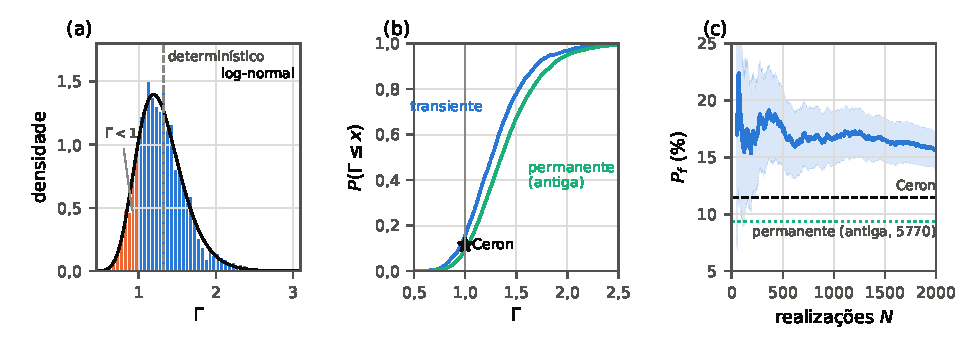
\includegraphics[width=\linewidth]{fig_rb_mc.pdf}
\caption{Monte Carlo direto com o transiente: (a) histograma de $\Gamma$ (em laranja, as falhas) e a log-normal
ajustada; (b) distribuição acumulada de $\Gamma$ com o transiente e na campanha antiga (permanente), com a $P_f$ do
Ceron em $\Gamma = 1$; (c) $P_f$ com o número de realizações e a faixa de 95\%.}\label{fig:mc}
\end{figure}

\subsection{O que leva à ruptura}
Cada realização grava as médias dos campos na banda de ruptura ($\sqrt{J_2(\varepsilon_p)} \geq \LimiarBanda$ do maior)
e a profundidade dela. A Tab.~\ref{tab:spearman} e a Fig.~\ref{fig:mecanismo} mostram:
\begin{itemize}
\item o $c'$ na banda domina: Spearman de \RhoC{} com $\Gamma$ (\ParcC{} descontados $\varphi'$ e $k_v$). As falhas
têm \FalhaC~kPa na banda, contra \OutrasC~kPa nas outras realizações;
\item $\varphi'$ e $k_v$ na banda vêm depois, com Spearman parcial de \ParcPhi{} e \ParcK. Dados $c'$ e $\varphi'$,
um $k_v$ menor na banda ainda baixa $\Gamma$: nas falhas, $k_v$ na banda vale \FalhaK{} da média, contra \OutrasK{}
nas outras;
\item as falhas têm banda um pouco mais funda (\FalhaProf{} contra \OutrasProf~m) e $p_w$ maior nela (\FalhaPw{}
contra \OutrasPw~kPa). O $k_v$ e o $p_w$ na banda têm Spearman de \RhoKPw, mas o $p_w$ também cresce com a
profundidade (\RhoPwProf). Separar o efeito do $k_v$ é o papel do teste pareado (Seção~\ref{sec:kfixo});
\item o mapa da banda nas falhas é parecido com o de todas as realizações: a banda sai da crista e chega ao pé, perto
da do determinístico. O mapa não mostra um segundo mecanismo.
\end{itemize}

\begin{table}[htbp]\centering\footnotesize
\caption{O que leva à ruptura: Spearman de $\Gamma$ com cada média na banda, Spearman parcial de 2ª ordem (Eqs.~70 e
71 do Ceron: cada variável descontadas as outras duas) e as médias nas falhas, nas outras realizações e no
determinístico.}\label{tab:spearman}
\begin{tabular}{lrrrrr}\toprule
média na banda & Spearman & parcial & falhas & outras & determinístico \\\midrule
$c'$ (kPa) & \RhoC & \ParcC & \FalhaC & \OutrasC & \DetC \\
$\varphi'$ (graus) & \RhoPhi & \ParcPhi & \FalhaPhi & \OutrasPhi & \DetPhi \\
$k_v$ (multiplicador) & \RhoK & \ParcK & \FalhaK & \OutrasK & \DetK \\
$p_w$ (kPa) & \RhoPw & -- & \FalhaPw & \OutrasPw & \DetPw \\
profundidade (m) & \RhoProf & -- & \FalhaProf & \OutrasProf & \DetProf \\
\bottomrule\end{tabular}\end{table}

\begin{figure}[htbp]\centering
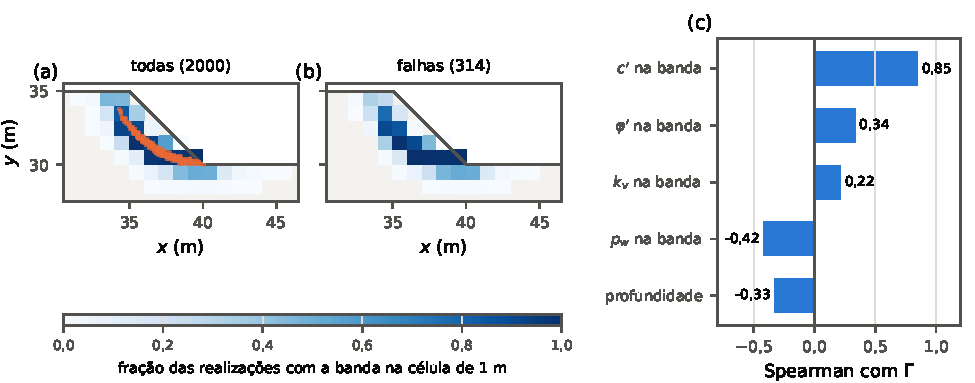
\includegraphics[width=\linewidth]{fig_rb_mecanismo.pdf}
\caption{Mecanismo: fração das realizações com a banda em cada célula de 1~m (\texttt{mc\_mapa\_*.csv}) em (a) todas,
com os pontos da banda do determinístico, e (b) nas falhas; (c) Spearman de $\Gamma$ com as médias na banda.}
\label{fig:mecanismo}
\end{figure}

\subsection{A malha}\label{sec:malha}
O \texttt{niveis} de cada realização guarda $\Gamma$ em cada nível do refinamento. A Tab.~\ref{tab:niveis} e a
Fig.~\ref{fig:malha} mostram que o resultado ainda depende da malha:
\begin{itemize}
\item o último nível muda $\Gamma$ em \UltimoNivel\% na média (\UltimoNivelDet\% no determinístico) e leva a $P_f$ de
\PfNivelDois\% para \PfNivelTres\%;
\item a razão entre as duas últimas variações da média é \RazaoNiveis. Se ela se mantiver, mais um nível mudaria
$\Gamma$ em \ExtrapQuatro\%, e a $P_f$ iria a uns \PfExtrapQuatro\%; o limite da série dá \ExtrapLimite\% e
\PfExtrapLimite\%. É uma estimativa grosseira, mas a sensibilidade é clara: $\Gamma$ 1\% menor em todas as realizações
dá $P_f = \PfMenosUm\%$, e 2\% menor dá \PfMenosDois\%;
\item a campanha antiga mostra o mesmo, com $P_f$ de \PfAntigaNivelDois\% no nível 2 e \PfAntigaNivelTres\% no 3. A
campanha da chuva já usa um nível a mais.
\end{itemize}
Então a diferença para o Ceron mistura o modelo e a malha. Conferir o nível 4 é barato (Seção~\ref{sec:sugestoes}).

\begin{table}[htbp]\centering\footnotesize
\caption{$\Gamma$ e $P_f$ por nível de refinamento do fator (o nível 3 é o resultado).}\label{tab:niveis}
\begin{tabular}{rrrrr}\toprule
& \multicolumn{3}{c}{transiente (PC)} & permanente (antiga) \\\cmidrule(lr){2-4}\cmidrule(lr){5-5}
nível & $\Gamma$ determinístico & $\bar\Gamma$ & $P_f$ (\%) & $P_f$ (\%) \\\midrule
0 & \DetNivelZero & \MediaNivelZero & \PfNivelZero & \PfAntigaNivelZero \\
1 & \DetNivelUm & \MediaNivelUm & \PfNivelUm & \PfAntigaNivelUm \\
2 & \DetNivelDois & \MediaNivelDois & \PfNivelDois & \PfAntigaNivelDois \\
3 & \DetNivelTres & \MediaNivelTres & \PfNivelTres & \PfAntigaNivelTres \\
\bottomrule\end{tabular}\end{table}

\begin{figure}[htbp]\centering
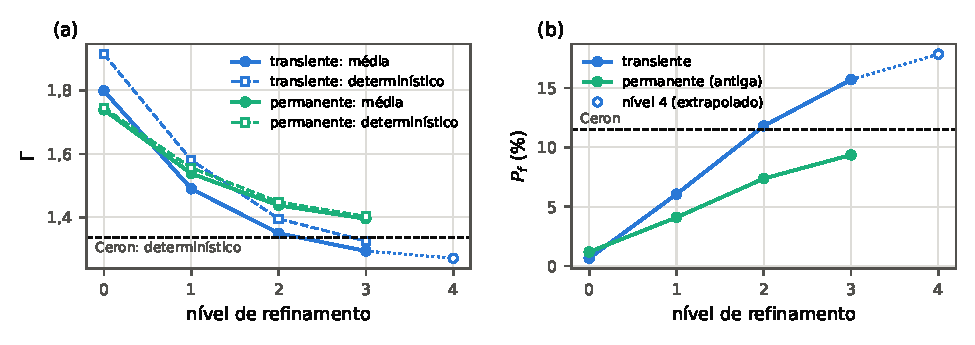
\includegraphics[width=\linewidth]{fig_rb_malha.pdf}
\caption{(a) $\Gamma$ por nível de refinamento: média das realizações e determinístico, com o transiente e na campanha
antiga; (b) $P_f$ por nível. Os círculos vazados são a extrapolação geométrica para o nível 4.}\label{fig:malha}
\end{figure}

\subsection{Comparação com o Ceron e com a campanha antiga}\label{sec:comparacao}
\begin{itemize}
\item \textbf{Ceron.} O \PfCeron\% do artigo fica fora do intervalo do direto (\PfDiretoLo\% a \PfDiretoHi\%), e os
dois intervalos não se tocam (Ceron: \PfCeronLo\% a \PfCeronHi\%). O $\Gamma$ determinístico e o $CoV(\Gamma)$ são
quase os mesmos, então a diferença de $P_f$ vem da posição da distribuição: a média fica \PosicaoDireto{} do
determinístico aqui e \PosicaoCeron{} no Ceron, e a média daqui (\GammaMedia) fica \MediaContraCeron{} da do Ceron
(\GammaMediaCeron). Com a média do Ceron e o CoV daqui, a log-normal daria $P_f = \PfLognCeron\%$, perto dos
\PfCeron\% do artigo. A malha pesa na mesma ordem (Seção~\ref{sec:malha}).
\item \textbf{Campanha antiga} (percolação permanente, no cluster). Ela dá $P_f = \PfAntiga\%$ em \NAntiga{}
realizações, com $\Gamma_{det} = \GammaDetAntiga$ e $\bar\Gamma/\Gamma_{det} - 1 = \MediaSobreDetAntiga\%$
(Tab.~\ref{tab:resumo}). O transiente tem $\Gamma_{det}$ menor e a média mais abaixo dele; o CoV é o mesmo.
\item \textbf{Sem pareamento.} As duas usam a semente \Semente{} e os mesmos $\xi$ na realização $n$, mas não o mesmo
retângulo da KL: \DomXAntiga~m $\times$ \DomYAntiga~m na antiga (a caixa da malha, \KLvarAntiga\% da variância) e
\DomX~m $\times$ \DomY~m aqui. Os modos são outros; só os maiores se parecem. Nas \NComuns{} realizações em comum, as
médias no solo todo têm correlação alta ($c'$: \CorrCmed; $\varphi'$: \CorrPhimed; $k_v$: \CorrKmed), mas o $c'$ na
banda não (\CorrBandaC), nem $\Gamma$ (\CorrGamma). A realização $n$ não é o mesmo talude nas duas campanhas, então a
comparação é só das distribuições. Ela também mistura o transiente com o domínio, a malha e o código.
\end{itemize}

\section{Amostragem por importância}\label{sec:ai}
\subsection{Os dois deslocamentos}
A teoria está na Seção~7 do \texttt{relatorio\_chuva.tex}: o estimador $\hat P_f = \frac1N\sum I_i w_i$, o peso exato
$w = \exp(-\xi\cdot\mu + \frac12|\mu|^2)$, por que ele não tem viés para qualquer $\mu$ fixado antes da amostra, e por
que o deslocamento tem de ter poucos graus de liberdade com \NVarKL{} variáveis (Au e Beck, 2003). O deslocamento é a média
dos $\xi$ das falhas do direto, a entropia cruzada de Rubinstein e Kroese (2004), regularizada de dois jeitos:
\begin{itemize}
\item \textbf{Na direção da banda} ($\mu_c = s_c\,d$, com $d$ a direção da banda do determinístico). Com as
\NfDireto{} falhas do direto, $s = (\SC;\ \SPhi;\ \SK)$ para $c'$, $\varphi'$ e $k_v$, e $|\mu|^2 = \MuDoisBanda$.
São três números, com ruído de uns $3/n_f = \RuidoBanda$.
\item \textbf{Nos primeiros modos} (a proposta da nota \texttt{form\_MIS/confiabilidade.tex}, Seção ``Amostragem por
importância sem gradiente''): a média dos $K = \KModos$ primeiros modos de cada campo nas mesmas falhas.
\ifmodosdesloc Ela tem $|\mu|^2 = \MuDoisModos$, mas só \MuDoisModosUtil{} disso está na direção da banda: os
\KModos{} primeiros modos guardam \DirecaoK\% de $|d|^2$. Os outros \MuDoisModosResto{} estão em outras direções. Se
eles não ajudarem, multiplicam o segundo momento do peso por $e^{\MuDoisModosResto} = \FatorRestoModos$. O ruído
esperado é só de $3K/n_f = \RuidoModos$: o resto inclui direções que a banda do determinístico não vê, e a AI nos
modos mostra se elas ajudam.\else O deslocamento ainda não foi calculado.\fi
\end{itemize}
Os dois deslocamentos foram fixados antes das amostras, com outras sementes (\SementeBanda{} e \SementeModos): as
amostras da AI são independentes do direto. A conferência dos pesos sem elementos finitos (\SorteiosBanda{} sorteios
com os deslocamentos de um piloto de \PilotoVerif{} realizações, \texttt{verificacao/}) dá peso médio de
$\PesoVerifBanda \pm \PesoVerifSeBanda$ na banda e $\PesoVerifModos \pm \PesoVerifSeModos$ nos modos, como deve ser
(1). O ganho esperado num estado limite linear com a $P_f$ do direto ($\beta = \BetaLinear$) é \GanhoLinear: o
deslocamento ótimo teria $|\mu|^2 = \MdoisLinear$, perto do \MuDoisBanda{} da banda.

\subsection{Resultados}
\ifaipronto As \NBanda{} realizações da AI na banda\else As \NBanda{} realizações da AI na banda feitas até agora (de
\NAlvoBanda; a rodada termina por volta de \FimBanda)\fi{} dão (Tab.~\ref{tab:ai}, Fig.~\ref{fig:ai}):
\begin{itemize}
\item $P_f = \PfBanda\%$, com $CoV(P_f) = \CovPfBanda\%$ e faixa de 95\% de \PfBandaLo\% a \PfBandaHi\%. A diferença
para o direto é de \DifBandaPontos{} ponto percentual, ou \DifBanda{} desvio: \ViesBanda;
\item \NfBanda{} falhas sorteadas (\FracFalhaBanda\%), contra \PfDireto\% no direto: o deslocamento põe a amostra na
região de falha. A média das projeções sorteadas, $(\ProjMediaBanda)$, é o deslocamento pedido;
\item os pesos das falhas são pequenos (média \PesoFalhaBanda, maior \PesoMaxBanda): nenhuma falha domina a soma. O
peso médio de todas é $\PesoMedioBanda \pm \PesoMedioBandaSe$, compatível com 1;
\item o tamanho efetivo da amostra, $(\sum w)^2/\sum w^2 = \EssBanda$, é pequeno por causa das realizações seguras do
lado oposto ao deslocamento, que têm peso grande (Fig.~\ref{fig:ai}c). Elas não entram na $P_f$; o que vale é o
$CoV(P_f)$;
\item \textbf{ganho:} com o mesmo $N$ e essa $P_f$, o direto teria $CoV(P_f) = \CovDiretoMesmoNBanda\%$. Para o
$CoV$ da AI, ele precisaria de \NDiretoParaCovBanda{} realizações, \GanhoBanda{} vezes mais. É \FracGanhoBanda\% do
ganho do estado limite linear (\GanhoLinear): $\Gamma$ não é linear nos $\xi$, e a direção da banda é uma aproximação.
\end{itemize}
A AI nos modos \ifmodospronto terminou: com \NModos{} realizações, $P_f = \PfModos\%$ ($CoV = \CovPfModos\%$),
\DifModos{} desvio do direto (\ViesModos), \NfModos{} falhas sorteadas e ganho de \GanhoModos, \ComparaGanho{} o da
banda.\else está \ifmodosiniciado rodando\else pendente\fi{} (termina por volta de \FimModos).\ifmodosiniciado{} Até
agora, com \NModos{} de \NAlvoModos{} realizações, $P_f = \PfModos\%$ ($CoV = \CovPfModos\%$), \DifModos{} desvio do
direto; ainda é cedo para comparar o ganho.\fi\fi

\begin{table}[htbp]\centering\footnotesize\setlength{\tabcolsep}{4.5pt}
\caption{Monte Carlo direto e AI. Falhas: realizações sorteadas com $\Gamma < 1$; ESS: $(\sum w)^2/\sum w^2$;
diferença: $(P_f^{AI} - P_f^{dir})$ em desvios; ganho: quantas vezes mais realizações o direto pediria para o mesmo
$CoV(P_f)$.}\label{tab:ai}
\begin{tabular}{lrrrrrrrr}\toprule
método & $N$ & falhas & peso médio & ESS & $P_f$ (\%) & $CoV(P_f)$ (\%) & diferença & ganho \\\midrule
Monte Carlo direto & \NDireto & \NfDireto & 1 & \NDireto & \PfDireto & \CovPfDireto & -- & 1 \\
\rotBanda & \NBanda & \NfBanda & \PesoMedioBanda & \EssBanda & \PfBanda & \CovPfBanda & \DifBanda & \GanhoBanda \\
\linhaModos
estado limite linear & -- & -- & -- & -- & -- & -- & -- & \GanhoLinear \\
\bottomrule\end{tabular}\end{table}

\begin{figure}[htbp]\centering
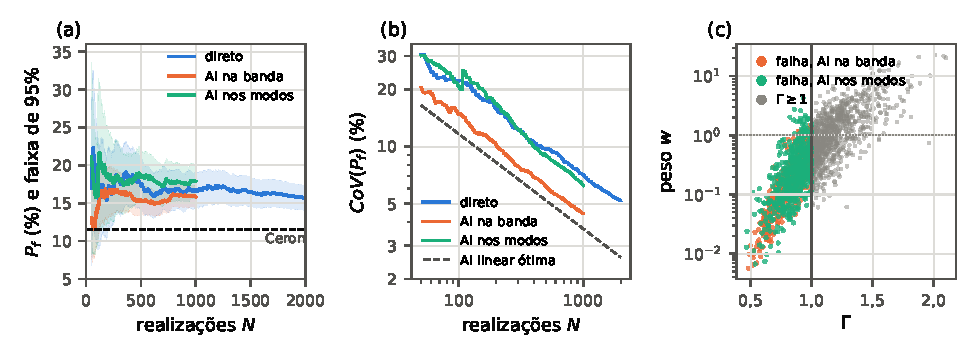
\includegraphics[width=\linewidth]{fig_rb_ai.pdf}
\caption{Direto e AI: (a) $P_f$ com o número de realizações e a faixa de 95\%; (b) $CoV(P_f)$, com a reta da AI no
estado limite linear com o deslocamento ótimo; (c) peso de cada realização da AI contra $\Gamma$.}\label{fig:ai}
\end{figure}

\subsection{Conclusão}
\begin{itemize}
\item A AI na direção da banda não mostra viés: ela concorda com o direto.
\item Com $P_f \approx \PfDireto\%$, o ganho é modesto (\GanhoBanda{} vezes), como a teoria prevê. Para a
referência do Ceron, o Monte Carlo direto basta, e ele dá também a distribuição de $\Gamma$ e o mecanismo.
\item A AI compensa com $P_f$ pequena: com \PfChuva\%, a $P_f$ esperada da chuva, o estado limite linear dá
\GanhoLinearUm{} vezes. É lá que ela deve ser usada (Seção~\ref{sec:sugestoes}).
\item \ifmodospronto Os modos dão ganho \ComparaGanho{} o da banda (\GanhoModos{} contra \GanhoBanda). Com
\MuDoisModosResto{} de $|\mu|^2$ fora da direção da banda, esperava-se que os modos rendessem menos.\else A
comparação dos dois deslocamentos fica para quando a AI nos modos terminar. Com \ifmodosdesloc \MuDoisModosResto{} de
$|\mu|^2$ fora da direção da banda,\else o deslocamento fora da direção da banda,\fi{} a expectativa é que os modos
rendam menos.\fi
\end{itemize}

\section{Teste com \texorpdfstring{$k_v$}{kv} fixo}\label{sec:kfixo}
O $k_v$ muda as pressões do transiente, e o Spearman parcial de \ParcK{} diz que ele pesa em $\Gamma$. A pergunta é
se ele explica a $P_f$ maior. O teste usa as mesmas \NAlvoKfixo{} realizações do direto, com os mesmos $c'$ e
$\varphi'$, e $k_v$ fixo ($CoV(k_v) = \CovKfixo$). A comparação é pareada (a lógica do
\texttt{covk0/compara\_pareado.py}):
\begin{itemize}
\item McNemar nas falhas discordantes (as realizações que falham só com um dos dois);
\item a diferença média de $\Gamma$, realização a realização.
\end{itemize}
No Ceron, o $k_v$ aleatório muda pouco a $P_f$: ela vai de \PfCeronKfixo\% com $k_v$ fixo para \PfCeron\% com
$CoV(k_v) = \CovK$, só \CeronDifK{} ponto, e $\bar\Gamma$ vai de \GammaMediaCeronKfixo{} para \GammaMediaCeron{}
(Tabelas~3 e~4). A campanha antiga já tem o mesmo teste com percolação permanente: $P_f = \AntPfFixo\%$ com $k_v$ fixo e \AntPfAleat\%
com $k_v$ aleatório, nas \AntNPar{} realizações pareadas. São \AntNzu{} falhas só com $k_v$ aleatório e \AntNuz{} só
com $k_v$ fixo, com McNemar $p \AntMcNemar$. Em regime permanente, o $k_v$ não muda a $P_f$ (com $k_v$ aleatório,
$\Gamma$ médio fica só $\AntDifGamma \pm \AntDifGammaSe$ maior).

\ifkfixopronto
\textbf{Resultado} (Tab.~\ref{tab:kfixo}, Fig.~\ref{fig:kfixo}). Nas \KNPar{} realizações, a $P_f$ vai de
\KPfFixo\% com $k_v$ fixo para \KPfAleat\% com $k_v$ aleatório. São \KNzu{} falhas só com $k_v$ aleatório e \KNuz{}
só com $k_v$ fixo: a diferença é de $\KDifPf \pm \KDifPfSe$ pontos, com McNemar $p \KMcNemar$. A diferença média de
$\Gamma$ (aleatório menos fixo) é $\KDifGamma \pm \KDifGammaSe$ (mediana \KDifGammaMediana), e $\Gamma$ é maior com
$k_v$ aleatório em \KMaisAleat\% das realizações. Ela tem Spearman de \KRhoBanda{} com o $k_v$ médio na banda e
\KRhoSolo{} com o do solo todo. \KConclusao

\begin{table}[htbp]\centering\footnotesize
\caption{Teste pareado: as mesmas realizações com $k_v$ fixo e aleatório (IC: Wilson, 95\%).}\label{tab:kfixo}
\begin{tabular}{lrrr}\toprule
caso & realizações & $P_f$ (\%) & IC (\%) \\\midrule
\linhaKfixoPronta
\bottomrule\end{tabular}\end{table}

\begin{figure}[htbp]\centering
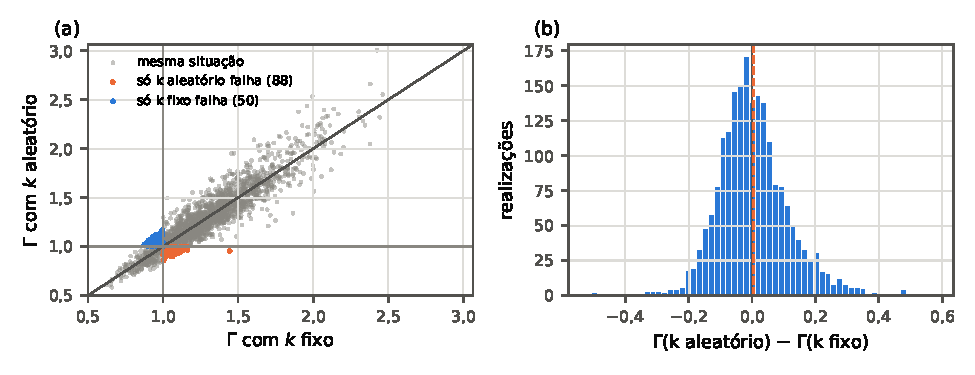
\includegraphics[width=\linewidth]{fig_rb_kfixo.pdf}
\caption{Teste pareado: (a) $\Gamma$ com $k_v$ aleatório contra $\Gamma$ com $k_v$ fixo, com as falhas discordantes;
(b) a diferença realização a realização.}\label{fig:kfixo}
\end{figure}
\else
\textbf{Resultado: pendente (termina por volta de \FimKfixo).} \ifkfixoiniciado A rodada começou às \InicioKfixo.
Até agora, com \KNPar{} realizações pareadas, a $P_f$ é de \KPfFixo\% com $k_v$ fixo e \KPfAleat\% com $k_v$
aleatório (\KNzu{} falhas só com $k_v$ aleatório e \KNuz{} só com $k_v$ fixo).\else A rodada começa quando a AI nos
modos acabar, por volta de \InicioKfixo.\fi{} Se o $k_v$ aleatório explicar a diferença, a $P_f$ com $k_v$ fixo deve
cair para perto dos \PfCeronKfixo\% do Ceron com $k_v$ fixo (Tabela~3) e as falhas discordantes devem pender para o
lado do $k_v$ aleatório.
\fi

\section{Campanhas no fermi}\label{sec:fermi}
\subsection{Os três solos (rodando)}
Os três solos de Rahardjo et al.\ (2007) rodam no fermi desde as \SolosInicio, com \SolosNos{} nós
(\texttt{CAMPANHA=solos}): Monte Carlo direto com $I = \SolosIks\,k_s$ por \SolosDuracao~h e o $FS$ do SRM (redução
da resistência) de \SolosPasso{} em \SolosPasso~h até \SolosFim~h. A
realização $n$ tem os mesmos campos nos três solos. O \texttt{status.sh} das \SolosHora{} (Tab.~\ref{tab:solos}):

\begin{table}[htbp]\centering\footnotesize
\caption{Os três solos no fermi às \SolosHora{} (\texttt{status.sh}, colado à mão): realizações, falhas e $P_f$ parcial
(IC de Wilson de 95\%), e o mínimo do $FS$ determinístico.}\label{tab:solos}
\begin{tabular}{lrrrrrr}\toprule
solo & $I$ (mm/h) & $N$ & feitas & falhas & $P_f$ parcial (\%) & $FS_{det}$ mínimo \\\midrule
$f_{10,-4}$ & \SolosIDez & \SolosNDez & \SolosFeitasDez & \SolosFalhasDez & \SolosPfDez{} (\SolosLoDez--\SolosHiDez) &
\SolosDetDez{} (\SolosTdetDez) \\
$f_{50,-5}$ & \SolosICinquenta & \SolosNCinquenta & \SolosFeitasCinquenta & \SolosFalhasCinquenta &
\SolosPfCinquenta{} (\SolosLoCinquenta--\SolosHiCinquenta) & \SolosDetCinquenta{} (\SolosTdetCinquenta) \\
$f_{100,-6}$ & \SolosICem & \SolosNCem & \SolosFeitasCem & \SolosFalhasCem & \SolosPfCem{} (\SolosLoCem--\SolosHiCem) &
\SolosDetCem{} (\SolosTdetCem) \\
\bottomrule\end{tabular}\end{table}

\begin{itemize}
\item São \SolosFeitasTotal{} de \SolosTotal{} realizações. A previsão é de mais \SolosPrevMin{} a \SolosPrevMax~h,
com o fim entre \SolosFimFaixa.
\item Os números são parciais: o \texttt{montecarlo.cpp} grava uma linha por instante, e o \texttt{status.sh} conta as
realizações em curso com os instantes já calculados. Nelas, o menor $FS$ ainda pode cair.
\item O esperado já aparece: o f10 rompe quase sempre (o determinístico fica abaixo de 1), o f100 quase nunca, e o f50
é o caso que discrimina.
\end{itemize}

\subsection{Campanhas prontas}
Os casos estão nos arquivos \texttt{cluster/casos*.txt}, e os comandos no \texttt{cluster/README.md}
(Tab.~\ref{tab:campanhas}). O custo usa \Nos{} nós $\times$ \Paralelo{} processos e um núcleo do fermi
\FermiLento{} vezes mais lento que o do PC: \CustoFermi~s por realização do rebaixamento.

\begin{table}[htbp]\centering\footnotesize\setlength{\tabcolsep}{4pt}
\caption{Campanhas do fermi: casos, realizações e custo (horas de CPU no fermi e de relógio com \Nos{} nós).}
\label{tab:campanhas}
\begin{tabular}{@{}L{2.5cm}L{4.2cm}L{2.3cm}rr@{}}\toprule
\texttt{CAMPANHA} & casos & $N$ & CPU (h) & relógio (h) \\\midrule
\texttt{solos} (rodando) & f10, f50 e f100, $FS$ até \SolosFim~h & \SolosTotal & -- & \SolosPrevMin--\SolosPrevMax{}
restantes \\
\texttt{chuva\_ai} & piloto e AI na banda, $I = \Iref$~mm/h, $FS$ de \ChuvaAITempos~h & \ChuvaAIPiloto{} +
\ChuvaAIN & -- & \ChuvaAIRelogio \\
\texttt{chuva}, fase 1 & referência, $FS$ em \ChuvaRefTempos~h & \ChuvaFaseUmN & \ChuvaFaseUmCpu & \ChuvaFaseUmRelogio \\
\texttt{chuva}, fase 2 & \ChuvaFaseDoisCasos{} casos: CoV, $s$ e $\alpha$ & \ChuvaFaseDoisN & \ChuvaFaseDoisCpu &
\ChuvaFaseDoisRelogio \\
\texttt{chuva}, fase 3 & \ChuvaFaseTresCasos{} intensidades & \ChuvaFaseTresN & \ChuvaFaseTresCpu &
\ChuvaFaseTresRelogio \\
\texttt{ceron} & direto, AI na banda e AI nos modos (piloto de \CeronPiloto) & \CeronDireto{} + \CeronBanda{} +
\CeronModos & \CeronCpu & \CeronRelogio \\
\bottomrule\end{tabular}\end{table}

\begin{itemize}
\item \texttt{solos}: \SolosMinReal~min por realização no fermi (\texttt{README.md}).
\item \texttt{chuva\_ai}: \ChuvaAIMin~min por realização (\texttt{casos\_chuva\_ai.txt}); o \texttt{README.md} espera
$CoV(P_f)$ de \ChuvaAICovLin\% a \ChuvaAICovMax\% com \ChuvaAIN{} realizações da AI.
\item \texttt{chuva}: a campanha inteira leva uns \ChuvaTotalDias{} dias; a fase~1 leva uns \ChuvaRelogioFaseUmReadme~h
de relógio por causa da cauda das tarefas (\texttt{README.md}).
\item \texttt{ceron}: o direto também é o piloto das duas AI (as \CeronPiloto{} primeiras realizações).
\end{itemize}

\section{Sugestões do que rodar}\label{sec:sugestoes}
\ifkfixopronto O PC ficou livre às \FimKfixo. O fermi fica ocupado até algo entre \SolosFimFaixa{} (três
solos).\else O PC fica ocupado até umas \FimKfixo{} (\ifmodospronto o $k_v$ fixo\else a AI nos modos e o $k_v$
fixo\fi), e o fermi, até algo entre \SolosFimFaixa{} (três solos).\fi{} Por ordem de prioridade
(Tab.~\ref{tab:sugestoes}):
\begin{enumerate}
\item \textbf{Malha, no PC, \ifkfixopronto que já está livre\else assim que ele liberar\fi.} O determinístico e as \SugMalhaN{} primeiras realizações com
\texttt{nref=4}, pareadas com as do direto (mesma semente). Numa pasta nova: cópias do \texttt{rodar.sh} e do
\texttt{bin/} do direto e uma pasta \texttt{logs/} (o \texttt{cluster/tarefas.sh} grava nela e não a cria); no
\texttt{casos.txt}, $N = \SugMalhaN$ (o do direto tem \NDireto) e \texttt{nref=4}; no \texttt{rodar.sh},
\texttt{BLOCO=\SugMalhaBloco}, para os \ProcPC{} processos dividirem as realizações. Com o fator umas duas vezes mais
caro, são \SugMalhaCusto~s por realização e uns \SugMalhaRelogio~min de relógio (o bloco que começa na realização 0
roda também o determinístico). O último nível ainda move a $P_f$ em pontos percentuais (Seção~\ref{sec:malha}), e a
resposta decide o \texttt{nref} de tudo o que vem depois. No mesmo determinístico vale conferir o passo de tempo: o
rebaixamento é \PassosTrans{} passo de \DtTrans~h, e o \texttt{rebaixamento\_mc.cpp} ainda não tem a opção
\texttt{dt=} (é preciso criá-la e passar o valor para o \texttt{DrawdownData::dt}).
\item \textbf{AI da chuva, no fermi, depois dos três solos} (\texttt{CAMPANHA=chuva\_ai}): piloto de \ChuvaAIPiloto{}
e AI de \ChuvaAIN{} realizações, com o $FS$ de \ChuvaAIPasso{} em \ChuvaAIPasso~h até \ChuvaAIFim~h; uns
\ChuvaAIRelogio~h com \Nos{} nós (\ChuvaAIRodadas{} rodadas de \ChuvaAIMin~min, porque a AI só começa quando o piloto
acaba). A referência da chuva tem $P_f \approx \PfChuva\%$, onde a AI rende mais: \GanhoLinearUm{} vezes no estado
limite linear, contra \GanhoLinear{} aqui na mesma conta (aqui a AI mediu \GanhoBanda).
\item \textbf{Seções 6.2 a 6.5 do Ceron com o transiente, no fermi.} Os casos da campanha antiga menos os de
$CoV(k_v)$, que vão para o item~4: CoV de $c'$ e $\varphi'$, $s$, $\alpha$ e $h_w/H$. São \SugCasos{} casos, com Monte
Carlo direto de \SugNporCaso{} realizações por caso: \SugBCpu~h de CPU e uns \SugBRelogio~h com \Nos{} nós com
\texttt{nref=3} (com \texttt{nref=4}, uns \SugBCpuQuatro~h e \SugBRelogioQuatro~h). Na campanha antiga, \SugDiretos{}
desses casos tiveram $P_f$ de \SugPfMinDireto\% a \SugPfMaxAntiga\%: neles o direto com \SugNporCaso{} realizações dá
$CoV(P_f) \leq \SugCovPfMax\%$. Os outros \SugPequenos, com $P_f < \SugLimiar\%$ (\SugPequenosLista), pedem AI: piloto
e AI com metade das realizações cada, no mesmo custo. Esses casos ainda não existem: as linhas entram no
\texttt{cluster/casos\_ceron.txt} na fase~2, como em ``Mais casos'' do \texttt{README.md}, e a submissão é
\texttt{CAMPANHA=ceron CASOS=fase2 ./submeter.sh \Nos}, para não rodar junto os \texttt{ref\_*} do item~6.
\item \textbf{Família de $CoV(k_v)$:} \SugKLista{} (os três últimos são os da Tabela~3 do Ceron), que
com o $k_v$ fixo e o direto dão \SugKPontos{} pontos. São \SugKN{} realizações: \SugKRelogioPC~h no PC ou
\SugKRelogioFermi~h no fermi. Se o teste da Seção~\ref{sec:kfixo} mostrar efeito, a família mostra como o $k_v$ age
no transiente; se não mostrar, ela só completa a Tabela~3 e pode esperar.
\item \textbf{Intensidade da chuva como variável aleatória:} a curva de fragilidade $P_f(I)$ com AI em \SugFragI{}
intensidades (uns \SugFragRelogio~h no fermi), depois integrada com a distribuição da chuva (IDF ou Gumbel), sem
elementos finitos.
\item \textbf{Opcional: a validação grande da AI no fermi} (\texttt{CAMPANHA=ceron}, uns \CeronRelogio~h). O PC não
mostrou sinal de viés da AI (\DifBanda{} desvio). A validação daria o ganho com mais precisão (\CeronBanda{}
realizações em cada AI), mas com um piloto menor que o do PC: \CeronPiloto{} realizações e umas \CeronPilotoFalhas{}
falhas, contra \NDireto{} e \NfDireto. Para um piloto maior, é preciso pôr \texttt{piloto\_n=\NDireto} nas duas linhas
\texttt{ref\_ai\_*} do \texttt{cluster/casos\_ceron.txt}.
\end{enumerate}

\begin{table}[htbp]\centering\footnotesize\setlength{\tabcolsep}{4pt}
\caption{Sugestões por ordem de prioridade, com o custo estimado.}\label{tab:sugestoes}
\begin{tabular}{@{}rL{4.6cm}lL{2.4cm}L{5.1cm}@{}}\toprule
& o quê & onde & custo & por quê \\\midrule
1 & malha: \texttt{nref=4}, determinístico e \SugMalhaN{} realizações & PC & \SugMalhaRelogio~min & a $P_f$ ainda depende
do último nível \\
2 & AI da chuva (\texttt{chuva\_ai}) & fermi & \ChuvaAIRelogio~h & $P_f \approx \PfChuva\%$: a AI rende mais \\
3 & Seções 6.2 a 6.5 com o transiente, sem os de $CoV(k_v)$ & fermi & \SugBRelogio{} a \SugBRelogioQuatro~h & o
artigo com o transiente \\
4 & $CoV(k_v)$ de \SugKLista & PC ou fermi & \SugKRelogioPC~h ou \SugKRelogioFermi~h & mais urgente se o $k_v$ fixo
mudar a $P_f$ \\
5 & fragilidade $P_f(I)$ com AI & fermi & \SugFragRelogio~h & a chuva como variável aleatória \\
6 & validação grande da AI (\texttt{ceron}) & fermi & \CeronRelogio~h & opcional \\
\bottomrule\end{tabular}\end{table}

\appendix
\section{Arquivos lidos e como atualizar}\label{sec:arquivos}
\raggedright As rodadas do PC estão em \path|~/projects/runs/ceron_transiente| (os caminhos abaixo são relativos a ela):
\begin{itemize}\small
\item direto: \path|direto/ceron_tr_fase1/f50_I0_iii/| (\path|mc_*.csv|, \path|mc_*.log|, \path|mc_mapa_*.csv|,
\path|mc_parametros.txt|), o determinístico em \path|direto/det/| (\path|mc_0_-1.csv| e \path|mc_real-1/|) e os
horários em \path|direto/logs/|;
\item AI na banda: \path|ai/desloc.txt|, \path|ai/casos.txt|, \path|ai/resultado.txt|, \path|ai/logs/| e
\path|ai/ceron_tr_fase1_ai/f50_I0_iii/|;
\item AI nos modos: \path|ai_modos/cadeia2.sh|, \path|ai_modos/falhas.txt|, \path|ai_modos/modos_desloc_modos.csv|,
\path|ai_modos/logs/| e \path|ai_modos/ceron_tr_fase1_ai_modos/f50_I0_iii/|;
\item $k_v$ fixo: \path|covk0/casos.txt|, \path|covk0/cadeia3.log| e \path|covk0/ceron_tr_covk0/f50_I0_iii/|;
\item pesos sem elementos finitos: \path|verificacao/| (\path|LEIAME.txt|).
\end{itemize}
A campanha antiga está em \path|~/projects/runs/fermi_ceron/ceron_mc|: \path|ceron_mc_fase1/f50_I0_iii/mc_resumo.csv|,
o determinístico em \path|ceron_mc_fase1/f50_I0_iii_det/|, o $k_v$ fixo em \path|ceron_mc_fase2/f50_I0_iii_covk0/| e os
outros casos em \path|ceron_mc_fase2/| e \path|ceron_mc_fase3/|; a malha, em
\path|Projects/LearningMohrCoulomb2/cluster/malhas/|. Das fontes: \texttt{rebaixamento\_mc.cpp},
\texttt{DrawdownTransient.h} e, em \texttt{cluster/}, \texttt{README.md}, \texttt{campanha.sh}, \texttt{submeter.sh} e
os \texttt{casos*.txt}; do build, \path|mc/serial_I24.log| (o custo da chuva).

Digitados no script: do Ceron, o $\Gamma$ determinístico (Fig.~24), as \NCeron{} simulações da referência
(Seção~6.1), a linha $s = 1$ da Tabela~4 e a linha $CoV(k_v) = 0$ da Tabela~3; o fator \FermiLento{} entre os núcleos
do fermi e do PC; e o \texttt{status.sh} dos três solos às \SolosHora.

\paragraph{Como atualizar.} Na pasta \texttt{relatorio/}:
\begin{verbatim}
python3 -I figuras_rebaixamento.py
pdflatex relatorio_rebaixamento.tex && pdflatex relatorio_rebaixamento.tex
\end{verbatim}
O script refaz as figuras e o \texttt{numeros\_rebaixamento.tex}. As chaves \texttt{\textbackslash ifaipronto},
\texttt{\textbackslash ifmodospronto} e \texttt{\textbackslash ifkfixopronto} ficam verdadeiras quando a rodada tem
todas as realizações e o \texttt{resultado.txt}; então o texto mostra os resultados no lugar de ``pendente''.

\begin{thebibliography}{9}
\bibitem{au2003} Au e Beck (2003). Importance sampling in high dimensions. \emph{Structural Safety} 25(2):139--163.
doi:10.1016/S0167-4730(02)00047-4.
\bibitem{rahardjo2007} Rahardjo, Ong, Rezaur e Leong (2007). Factors controlling instability of homogeneous soil slopes
under rainfall. \emph{Journal of Geotechnical and Geoenvironmental Engineering} 133(12):1532--1543.
doi:10.1061/(ASCE)1090-0241(2007)133:12(1532).
\bibitem{rubinstein2004} Rubinstein e Kroese (2004). \emph{The Cross-Entropy Method}. Springer, Nova York.
doi:10.1007/978-1-4757-4321-0.
\bibitem{ceron2025} Vargas Ceron, Cecílio, Linn e Maghous (2025). Stability analysis of slope subjected to seepage forces
considering spatial variability of soil properties. \emph{International Journal for Numerical and Analytical Methods in
Geomechanics} 49(11):2459--2491. doi:10.1002/nag.3993.
\end{thebibliography}
\end{document}
